% !TEX root = ../main.tex

\chapter{Model for metabolic age prediction} \label{chap:frassoni}
% Frassoni sani + CCS

%Per rispondere alla richiesta di Samuele:
%- MDA (malondialdeide) è un marcatore della perossidazione lipidica, quindi dello stress ossidativo
%- Consumo d'ossigeno e ATP sintesi con P/M: valutazione del consumo di ossigeno e sintesi di ATP in presenza di piruvato e malato che stimolano la via mitocondriale composta da Complesso I, III e IV (valuta la funzionalità del mitocondrio)
%- Consumo d'ossigeno e ATP sintesi con succinato: valutazione del consumo di ossigeno e sintesi di ATP in presenza di succinato che stimola la via mitocondriale composta da Complesso II, III e IV (valuta la funzionalità del mitocondrio)
%- ATP: concentrazione intracellulare di ATP
%- AMP: concentrazione intracellulare di AMP
%- ATP/AMP: rapporto tra le due precedenti  misure che indica lo stato energetico cellulare ( più elevato più la cellula possiede energia)
%- LDH: attività della lattico deidrogenasi, ultimo enzima del pathway della glicolisi anaerobia (antagonista della fosforilazione ossidativa che noi valutiamo tramite i consumo d'ossigeno e la sintesi di ATP).

\begin{displayquote}
	\textit{In this chapter, we evaluate the changes of energy metabolism during the physiological aging. To this aim we will develop a ML model that predicts the age of an individual starting from the following molecular biomarkers: oxidative phosphorylation efficiency, the \ac{ATP}/\ac{AMP} ratio, the lactate dehydrogenase activity and the level of malondialdehyde.  For this purpose we employed mononuclear cells obtained from healthy population with age between $5$ and $106$ years.} \todo{rewrite the abstract}
\end{displayquote}

\section{Introduction: aging and metabolism} \label{sec:frassoni_intro}

In this chapter we present the first biomedical data science challenge of the thesis.
This consists in devising a ML model capable of predicting the age of an individual starting from a set of molecular biomarkers collected from $118$ volunteers\footnote{this was referred to as \textit{the aging problem} throughout Chapter~\ref{chap:state-of-the-art}}.
This chapter describes the extensive EDA and the thorough model selection procedure which lead to the development of the final model.
Before diving into the details of the experimental setup, let's see some preliminary biological notions of how aging influences our metabolism.

Aging is a multifactorial process characterized by a progressive decline of physiological functions~\cite{campisi2013aging} which leads to an increment of vulnerability and the relative risk of disease and death ~\cite{bratic2010mitochondrial}.

Aging represents the primary risk factor for several chronic pathologies, such as cancer, cardiovascular disorders, diabetes and neurodegeneration~\cite{lopez2013hallmarks}. Different molecular pathways seem involved in the aging process, including deregulated autophagy, mitochondrial dysfunction, telomere shortening, oxidative stress, systemic inflammation and metabolism dysfunction~\cite{lopez2013hallmarks, riera2016signaling}.

Recently, an involvement of epigenetic modifications has been proposed~\cite{thompson2017epigenetic}, developing an \textit{aging clock} based on the degree of DNA methylation, which increases with the age~\cite{horvath2013dna}. However, for several years, aging has been considered the result of damages accumulation due to an excessive production of reactive oxygen species.

The \textit{Mitochondrial Theory of Aging}~\cite{harman1972biologic, sastre2000mitochondrial} derives from the  concept that mitochondria are the main source of oxidative stress~\cite{cadenas2000mitochondrial, turrens2003mitochondrial, dai2014mitochondrial} and the fact that mitochondrial DNA displays a
great rate of mutation together with a less efficient repair machinery with respect to nuclear DNA~\cite{short2005decline}. After some mitochondrial DNA mutation threshold, irreversible oxidative damages propagate throughout the genome. This phenomenon leads to dysfunction of mitochondrial metabolism~\cite{genova2004mitochondrial} accelerating the oxidative stress production~\cite{wallace2010mitochondrial}.

As shown in~\cite{mckerrell2015leukemia}, mononuclear cells isolated from peripheral blood, are an excellent model to evaluate the metabolic status of an entire organism. In fact, the molecular alterations identified in peripheral blood cells of aged normal subjects are statistically correlated with degenerative diseases~\cite{jaiswal2014age}.


\section{Data collection} \label{sec:frassoni_data_collection}

The study presented in this chapter is performed on mononuclear cells isolated from peripheral blood obtained from a population of $118$ volunteers\footnote{all participants provided their written informed consent to participate in this study, which was approved by the Ethics Committee of the IRCCS Istituto G. Gaslini, Genoa, IT, \todo{(N°)}} with age between $8$ and $106$ years.
In order to preserve the collected blood samples, the vacutainer tubes were transferred into the laboratory and analyzed within $24$ hours from collection.
All chemicals were purchased from Sigma Aldrich (St. Louis, MO, USA) and Ultrapure water (Milli-Q; Millipore, Billerica, MA, USA) was used throughout. All other reagents were of analytical grade.
Data collection and further analysis were managed by a team of specialized biologists at the IRCCS Istituto G. Gaslini, Genoa, IT. The following quantities were measured, on each blood sample.

\begin{itemize}
	\item[] \textbf{ATP} This complex molecule is the main responsible for storing and exchanging energy in cells and it is often referred to as the \textit{energy currency} of the cell. From a chemical point of view, ATP is made of an adenine base attached to a ribose sugar, which, in turn, is attached to three phosphate groups.
	ATP is heavily involved in the cellular aerobic respiration pathway. High levels of ATP correspond to high energetic state.
	ATP intracellular concentration, measured in $\text{mM}/\text{ml}$, is an important molecular biomarker to evaluate the energetic state of a cell.
	
	\item[] \textbf{AMP} This molecule is one of the main derivatives of ATP. In fact, AMP ca be obtained when two phosphate groups are removed from ATP, releasing energy that can be transferred to other molecules to trigger further cell reactions.
	So, when a cell is in good health, \ie high energetic level, AMP is low and ATP is high.
	AMP intracellular concentration is measured in $\text{mM}/\text{ml}$ and it is considered as an important molecular biomarker for the cellular energetic state. ATP and AMP quantification was based on the enzyme coupling method presented in~\cite{ravera2013tricarboxylic}.
%	as a side product of the ATP synthesis process or 
	
	\item[] \textbf{ATP/AMP ratio} Measuring ATP and AMP cellular concentration may not be enough to predict the age of an individual by assessing the energetic state of the peripheral blood cells. A more representative and interesting quantity can be their ratio, so ATP/AMP ratio was calculated and added to the feature set.
	
	\item[] \textbf{Oxygen consumption} Aerobic cellular respiration requires oxygen to produce ATP. Therefore, the cellular oximetric level is an important molecular biomarker for the metabolic assessment. Oxygen consumption was measured with an amperometric electrode in a closed chamber, magnetically stirred, at 37°C. The oxygen consumption measure, expressed in $\text{nmol~O}_2/(\text{min}\cdot\text{mg})$, is repeated in two versions, adding two different substrates, \ie:
	\begin{enumerate*}[label=(\roman*)]
		\item a combination of $5~\text{mM}$ pyruvate with $2.5~\text{mM}$ malate or
		\item only $20~\text{mM}$ succinate.
	\end{enumerate*}
	In the first oximetric measure, which from now on will be referred to as \copyrmal, the substrate stimulates the pathway composed by Complexes I, III and IV. On the other hand, in the second oximetric measure, which we call \cosucc, the substrate activates the pathway composed by Complexes II, III and IV, as described in~\cite{cappelli2017defects}.
	
	\item[] \textbf{ATP synthesis} We already covered the importance of ATP to evaluate the metabolic state of cells. So, we also measured ATP synthesis, expressed in $\text{nmol~ATP}/(\text{min}\cdot\text{mg})$,  by the highly sensitive luciferin/luciferase method. The same two substrates used for the oximetric evaluation were adopted. In the remainder of the chapter we refer to such measures as \atppyrmal and \atpsucc, accordingly.
	
	\item[] \textbf{P/O ratio} In order to assess the efficiency of oxidative phosphorylation, we also evaluated the ratio between ATP synthesis and oxygen consumption under both the substrates. We call the two obtained features as \popyrmal and \posucc, respectively.
	
	\item[] \textbf{Glycolytic flux} In order to assay the glycolytic flux, we measured the activity of the Lactate Dehydrogenase (\ac{LDH}), expressed in $\text{U}/\text{mg}$. This enzyme is important to evaluate the other metabolic pathway not mentioned so far, \ie the anaerobic respiration.
	
	\item[] \textbf{Lipid peroxidation} The uncoupled oxidative phosphorylation metabolism is often associated with an increment in the oxidative stress production~\cite{dai2014mitochondrial}, which induces damages on proteins, nucleic acid and membrane. Therefore, we evaluated the level of malondialdehyde (\ac{MDA}) as a marker of lipid peroxidation. The measure of \mda follows the protocol in~\cite{ravera2015oxidative}.
\end{itemize}

Each sample of this dataset is then described by the $12$-dimensional feature set summarized in Table~\ref{tab:aging_features}.

\begin{table}[]
	\centering
	\caption{The $12$-dimensional feature set.}
	\label{tab:aging_features}
	\begin{tabular}{@{}ll@{}}
		\toprule
		\textbf{Measure}                                    & \textbf{Feature name}\\ \midrule
		Gender of the individual                      & gender          \\
		ATP intracellular concentration            & \atp         \\
		AMP intracellular concentration            & \amp         \\
		ATP/AMP ratio                              & \atpamp      \\
		Oxygen consumption under Pyruvate + Malate & \copyrmal    \\
		Oxygen consumption under Succinate         & \cosucc      \\
		ATP synthesis under Pyruvate + Malate      & \atppyrmal   \\
		ATP synthesis under Succinate              & \atpsucc     \\
		P/O ratio under Pyruvate + Malate          & \popyrmal    \\
		P/O ratio under Succinate                  & \posucc      \\
		Glycolytic flux                            & \ldh         \\
		Lipid peroxidation                         & \mda         \\ \bottomrule
	\end{tabular}
\end{table}


\section{Exploratory data analysis} \label{sec:frassoni_EDA}
% BOXPLOT - PCA - HEATMAP etc
In this section we investigate on the relationship between the collected molecular biomarkers and the age of $118$ healthy individuals which volunteered to participate to this study.
Unfortunately, $7$ subjects presented missing values (in the features \ldh and sex). These subjects were excluded from EDA.


The data collection process entirely ran on voluntary basis. So, it is interesting to investigate on the resulting age distribution. As we can see from the histogram in Figure~\ref{fig:frassoni_agehist}, the decades of age are not equally represented. Ideally, we would have collected samples uniformly distributed with respect to their age, but this was unfortunately not possible.
%Therefore, we shall provide appropriate countermeasures to avoid bias in the following supervised regression step \todo{false so far}.

\begin{figure}[]
	\centering
	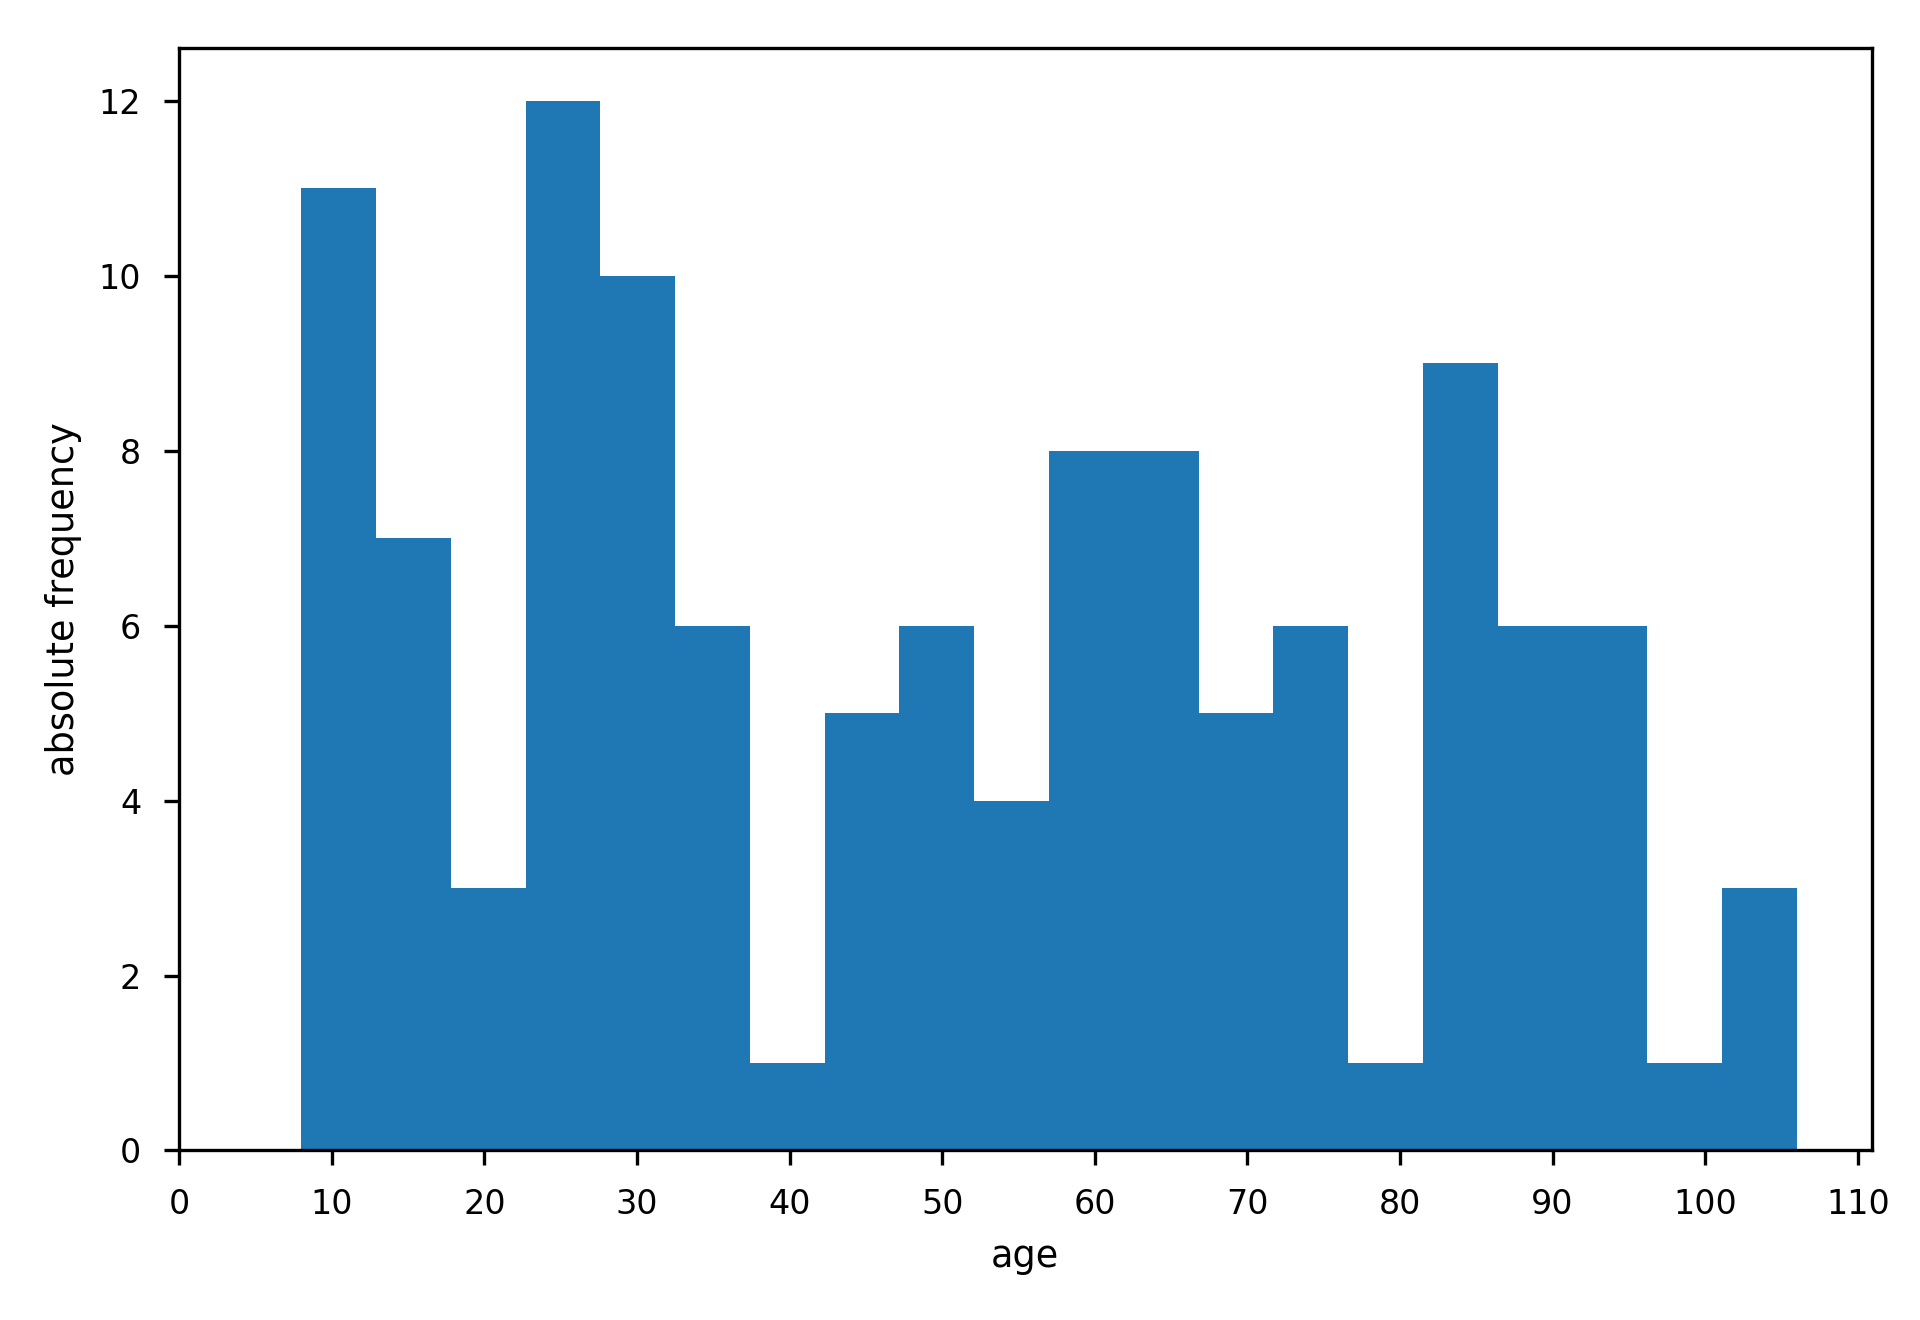
\includegraphics[width=0.8\textwidth]{part2/aging_agehist.png}
	\caption{Age distribution of the $118$ individuals involved in the study.} \label{fig:frassoni_agehist}
\end{figure}

Next, we aim at investigating on how the distribution of the molecular biomarkers is influenced by the age of individuals. To this aim we group the measures per decade and we represent their distribution with boxplots, see Figure~\ref{fig:frassoni_boxplot}.
As we can see, most of the biomarkers are clearly influenced by the age.
Let's start the visual inspection focusing on the variables related to the mitochondrial aerobic metabolism (from Figure~\ref{fig:frassoni_boxplot_copyrmal} to \ref{fig:frassoni_boxplot_atpamp}).
In particular, focusing our attention on the \atpamp ratio (Figure~\ref{fig:frassoni_boxplot_atpamp}), which is known to be an energy status monitor of the cells, we can see that the values decrease progressively with the decades, with a drastic drop between $40$ and $50$ years. Moreover, from an observation of \atp and \amp intracellular concentration (Figure~\ref{fig:frassoni_boxplot_atp} and Figure~\ref{fig:frassoni_boxplot_amp}, respectively) we can sense how the decrease of the \atpamp ratio is mainly due to the growth of \amp in the aging process.
Similar considerations can be made for the efficiency of oxidative phosphorylation, evaluated by \popyrmal and \posucc. In particular, \popyrmal oscillates around its reference level of $2.5~\text{nmol~O}_2/(\text{min}\cdot\text{mg})$~\cite{hinkle2005p} in subjects having from $0$ to $30$ years starting to decrease afterwards. Moreover, \popyrmal, similarly to \atpamp, is fairly stable at its lowest level for elderly (age $\geq 70$).
Let's now focus on the activity of LDH (Figure~\ref{fig:frassoni_boxplot_ldh}). As we can see, this metabolic biomarker almost monotonically increases with the aging process.
This is mainly due to the fact that LDH is involved in the glycolysis metabolism, which is a metabolic pathway chosen by the cell to compensate its altered aerobic metabolism.
Finally, let's focus on the distributions of the \mda (Figure~\ref{fig:frassoni_boxplot_mda}). As expected, \mda has an opposite trend with respect to \atpamp and \popyrmal. In fact, it increases from $21$ to $80$ years. This can be due to the increased oxidative stress production induced by uncoupled oxidative phosphorylation~\cite{dai2014mitochondrial}.
\mda is more stable for elderly, mainly because of their physiological metabolic slowdown.

\begin{figure}[]
	\centering
	\subfloat[]{%
		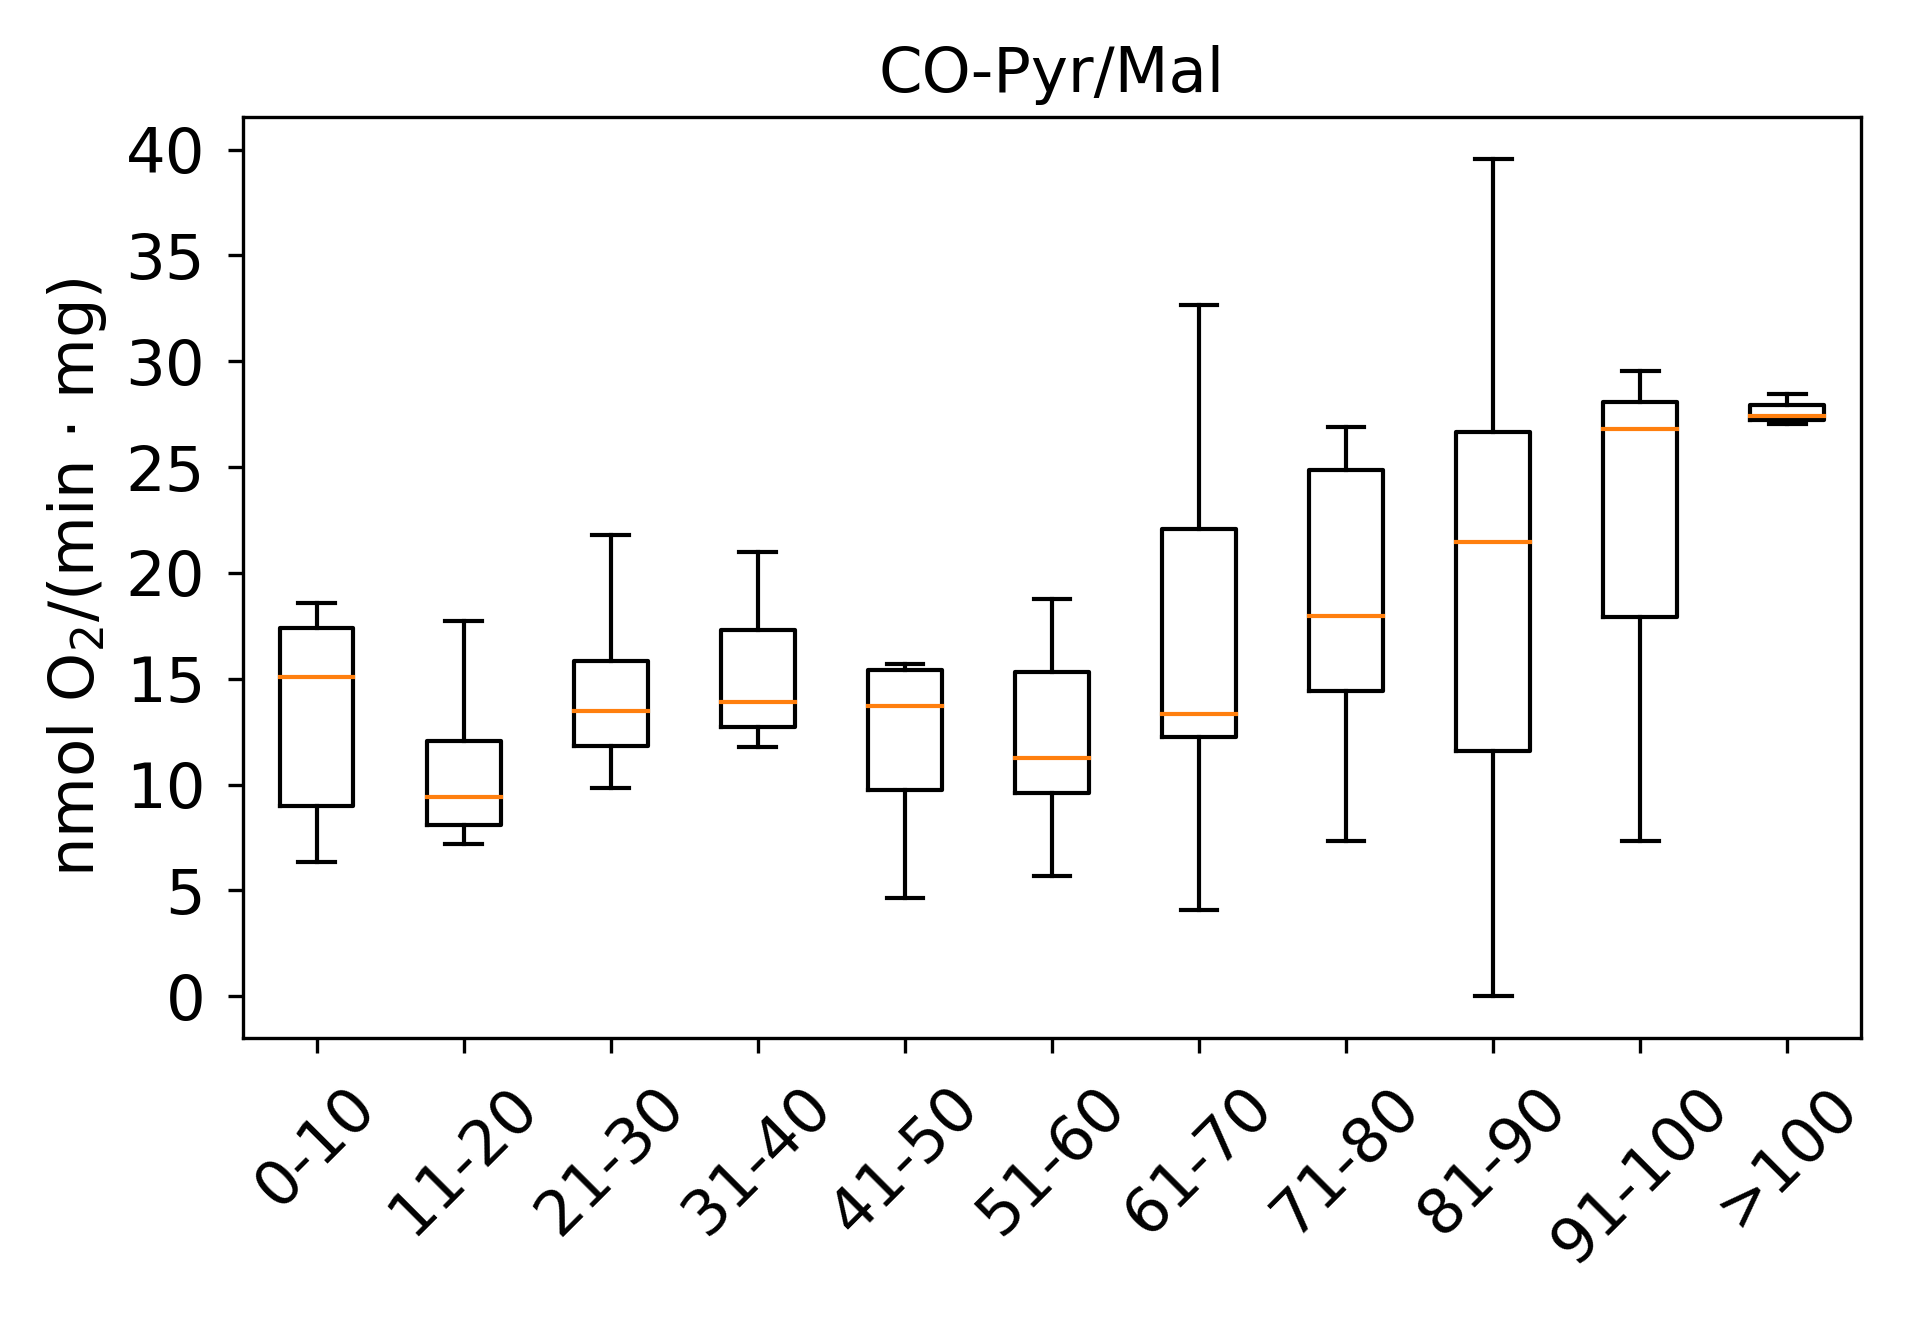
\includegraphics[width=0.33\textwidth]{part2/aging_boxplot_CO-PyrMal.png}
		\label{fig:frassoni_boxplot_copyrmal}%
	}%
	\subfloat[]{%
		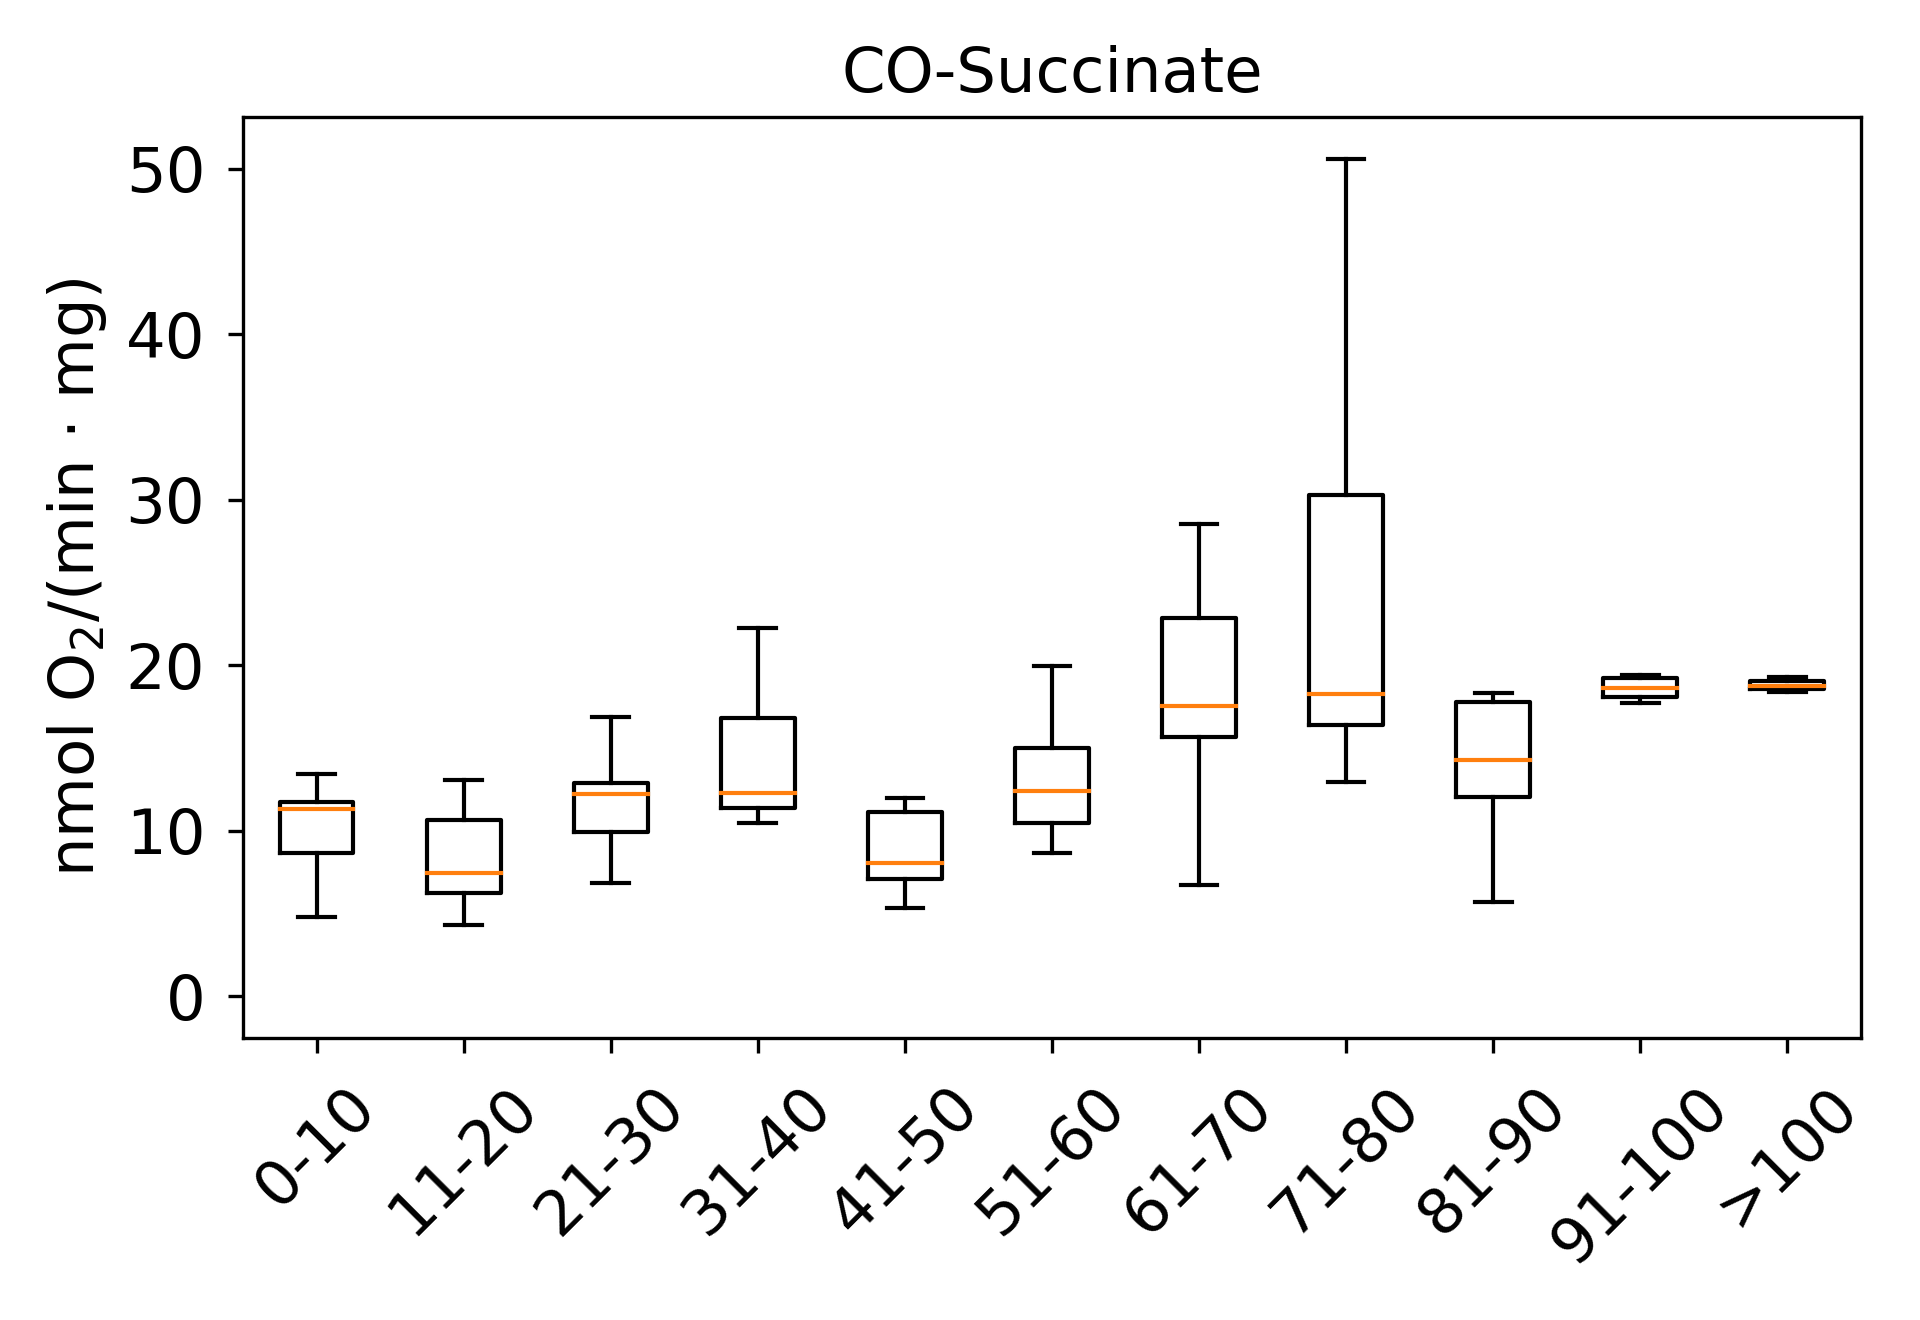
\includegraphics[width=0.33\textwidth]{part2/aging_boxplot_CO-Succinate.png}
		\label{fig:frassoni_boxplot_cosucc}%
	}%
%	\hfill%
	\subfloat[]{%
		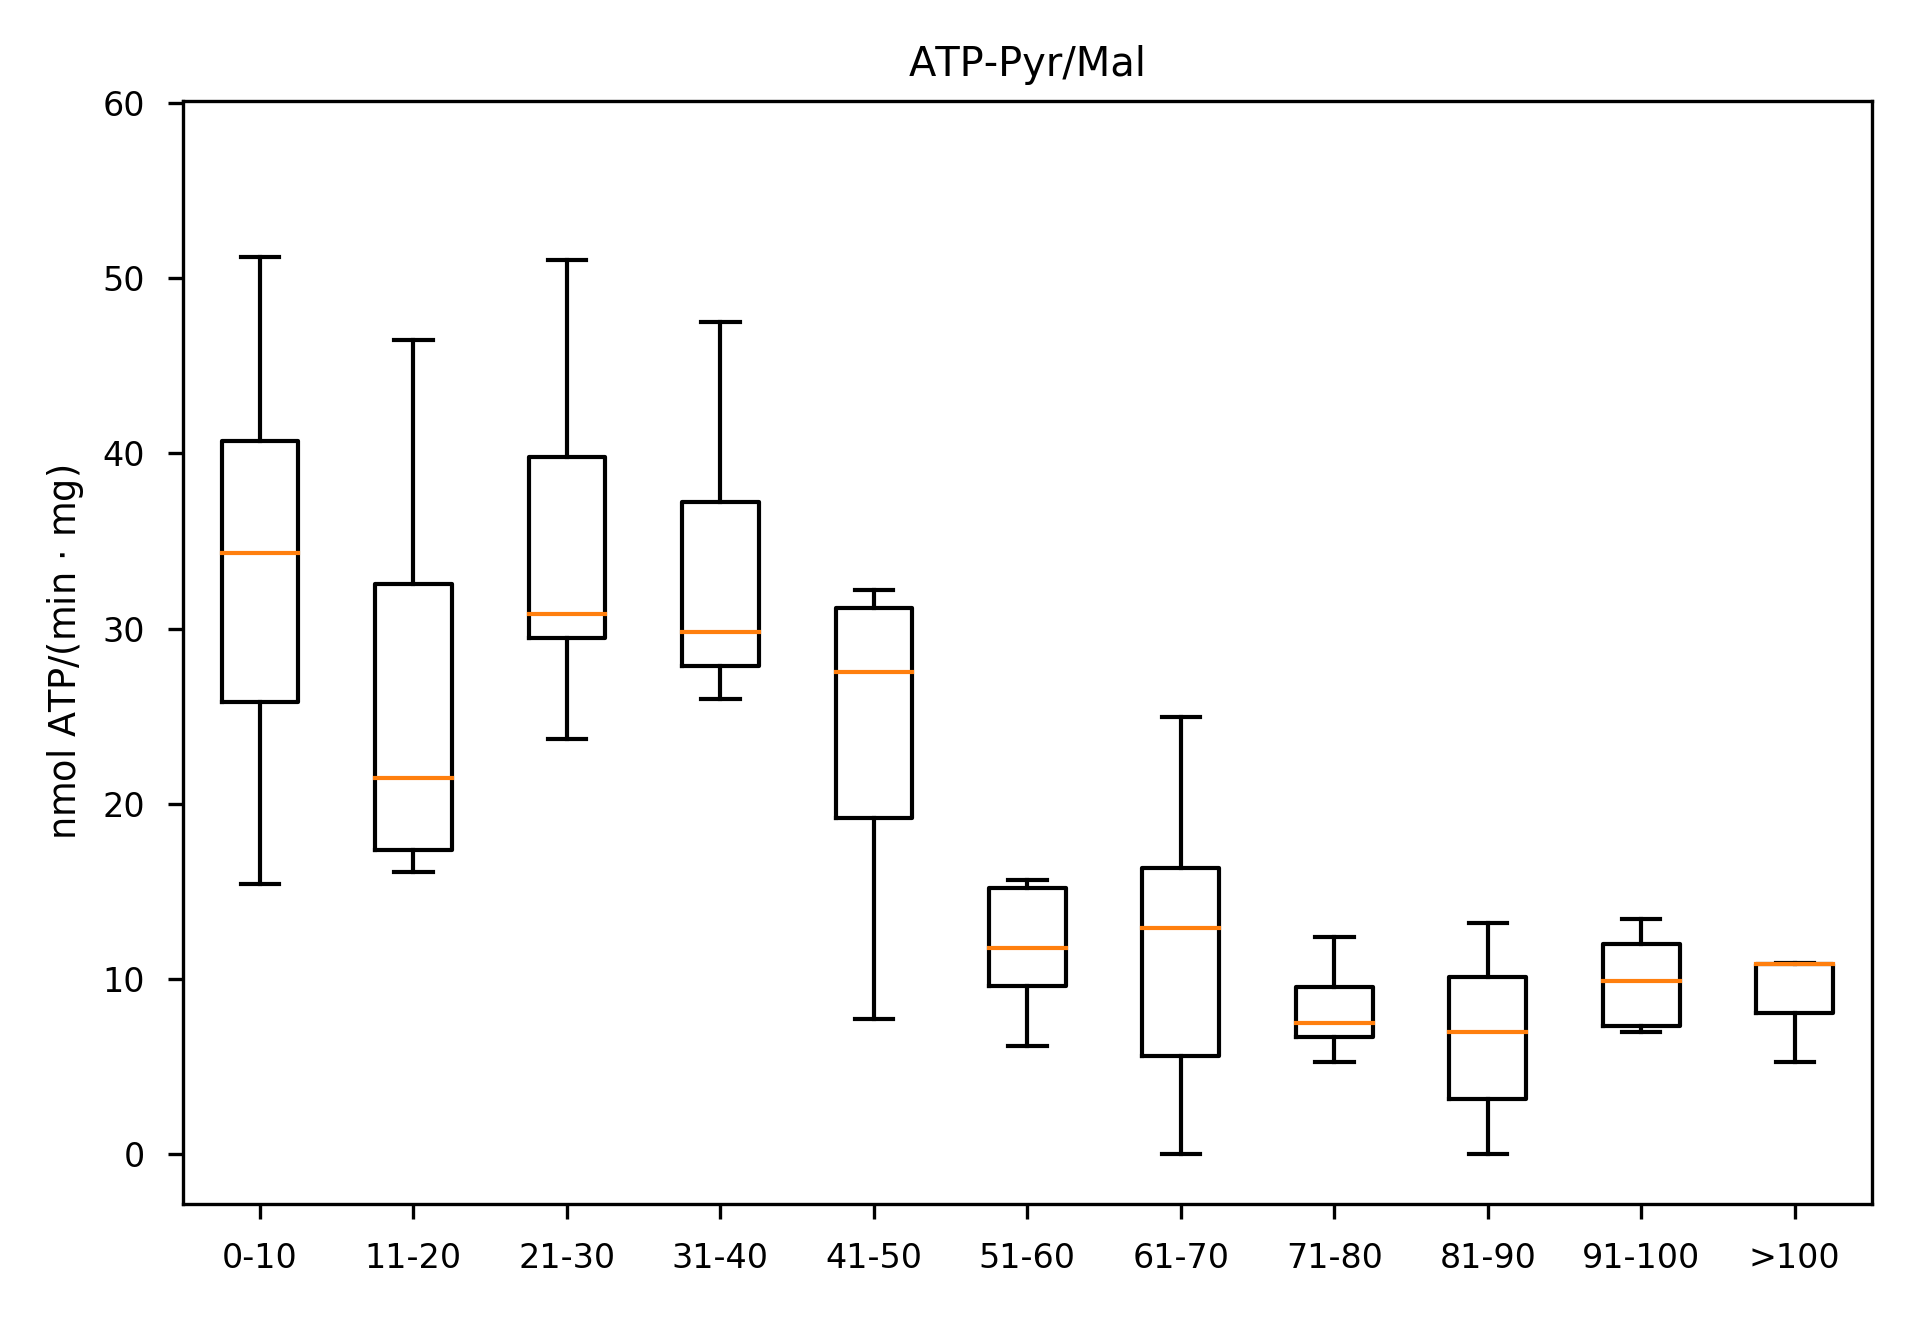
\includegraphics[width=0.33\textwidth]{part2/aging_boxplot_ATP-PyrMal.png}
		\label{fig:frassoni_boxplot_atppyrmal}%
	}%
	\hfill% %%%% ROW 2
	\subfloat[]{%
	   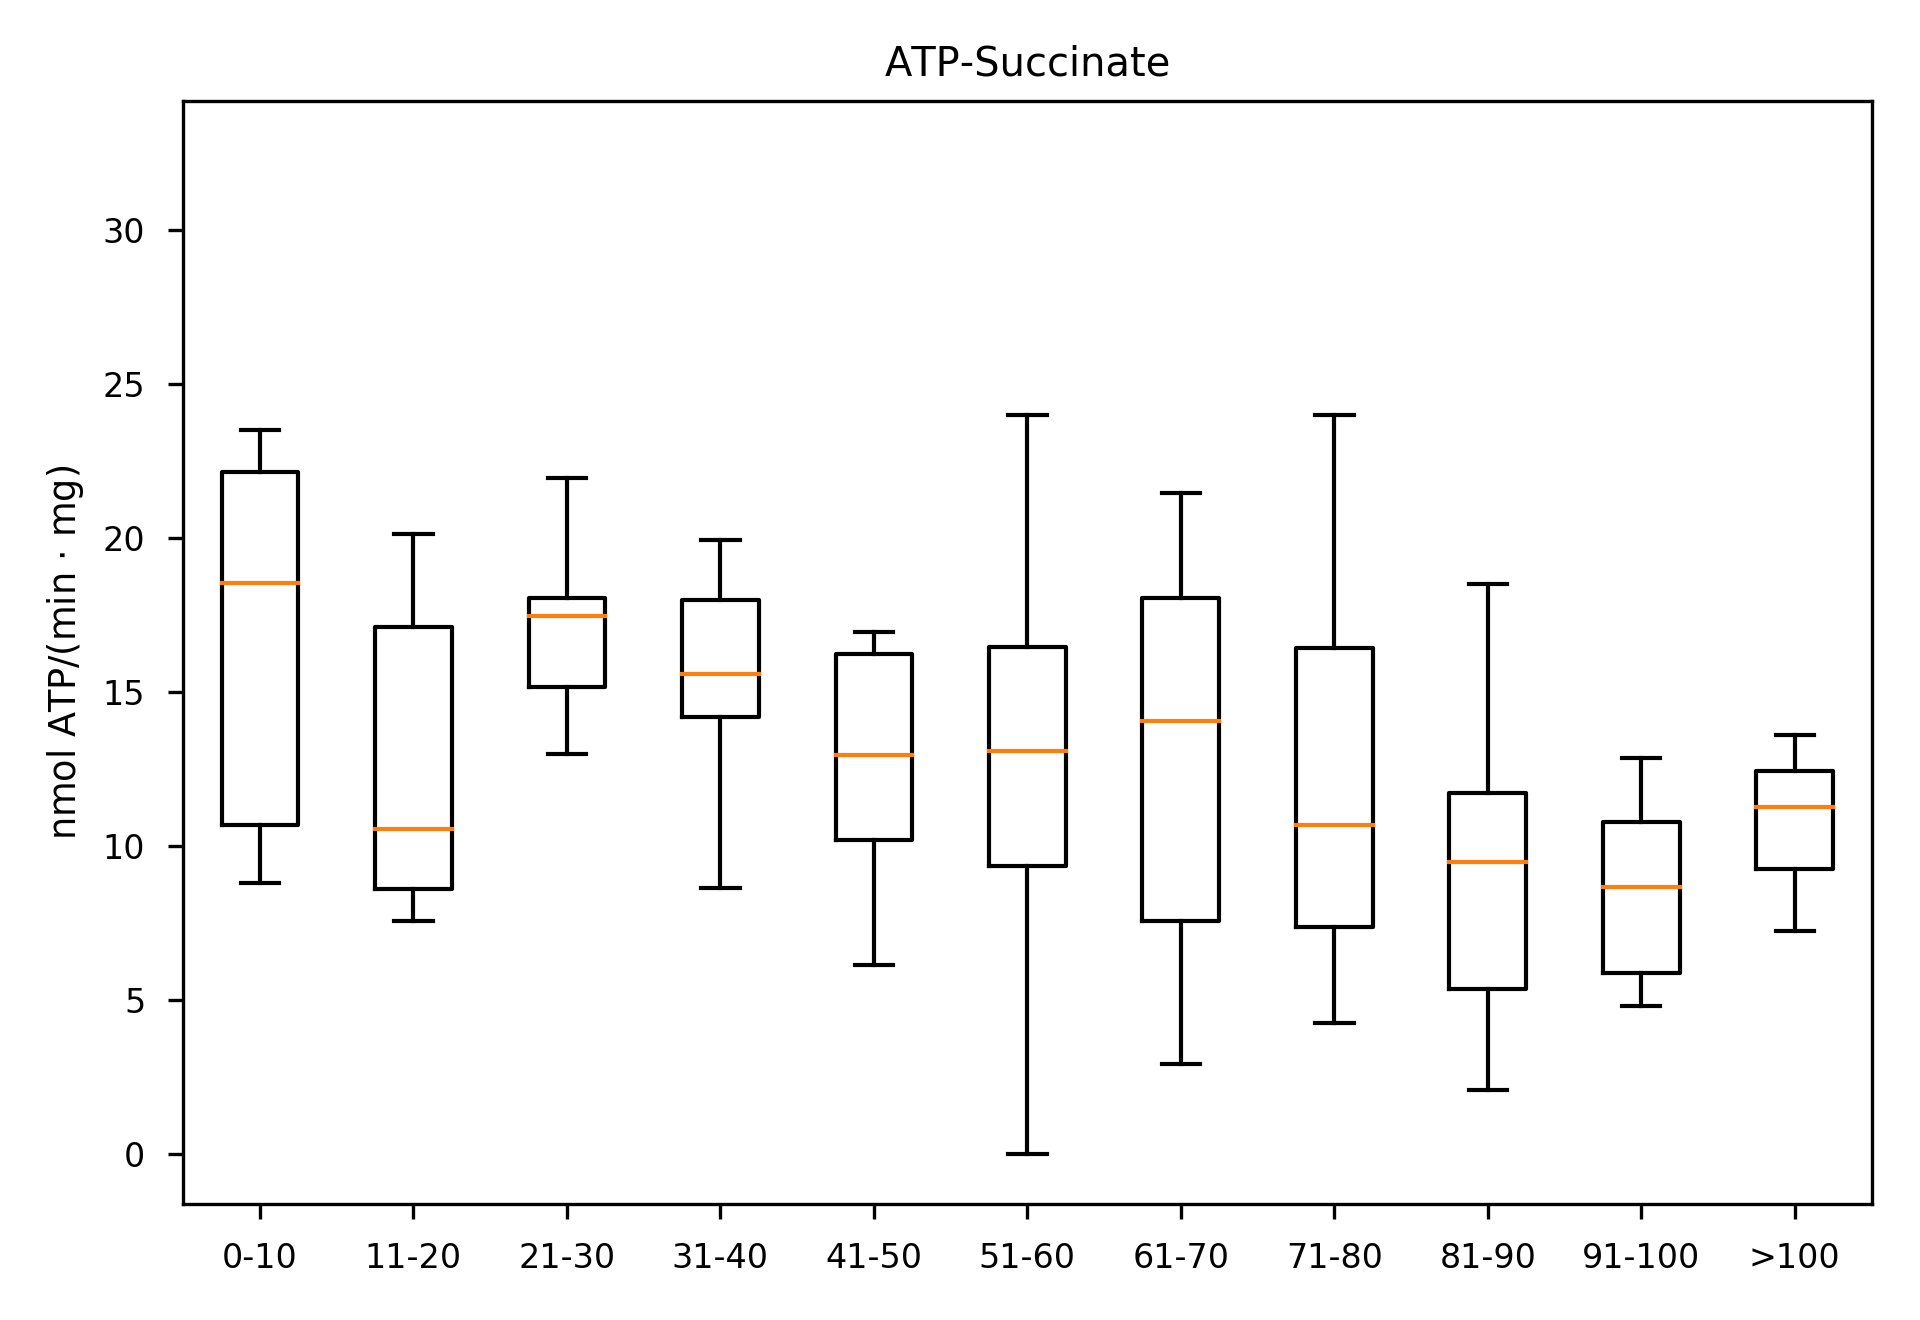
\includegraphics[width=0.33\textwidth]{part2/aging_boxplot_ATP-Succinate.png}
       \label{fig:frassoni_boxplot_atpsucc}%
	}%
	\subfloat[]{%
		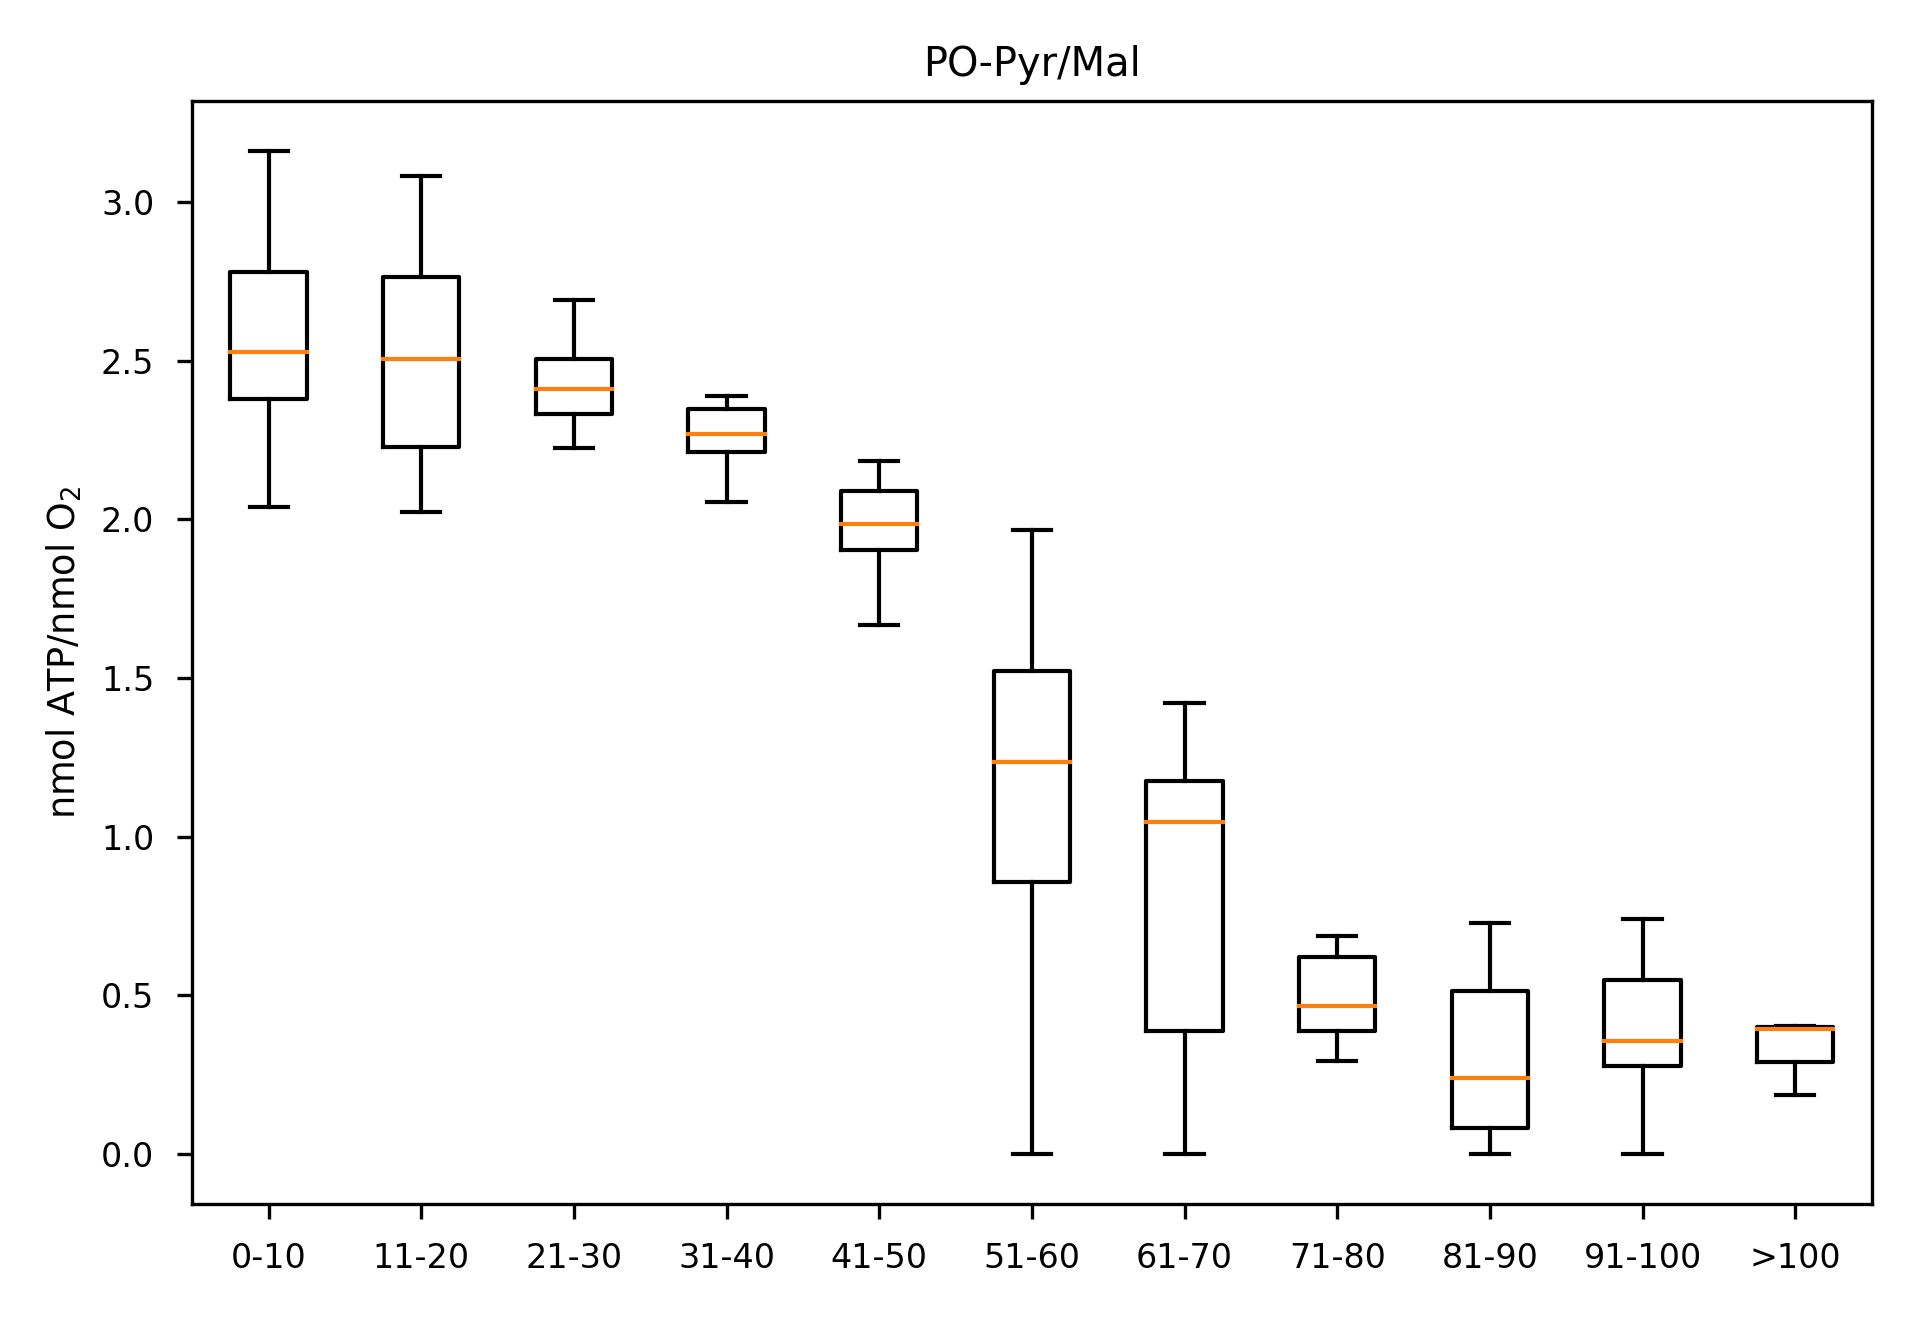
\includegraphics[width=0.33\textwidth]{part2/aging_boxplot_PO-PyrMal.png}
		\label{fig:frassoni_boxplot_popyrmal}%
	}%
	%	\hfill%
	\subfloat[]{%
		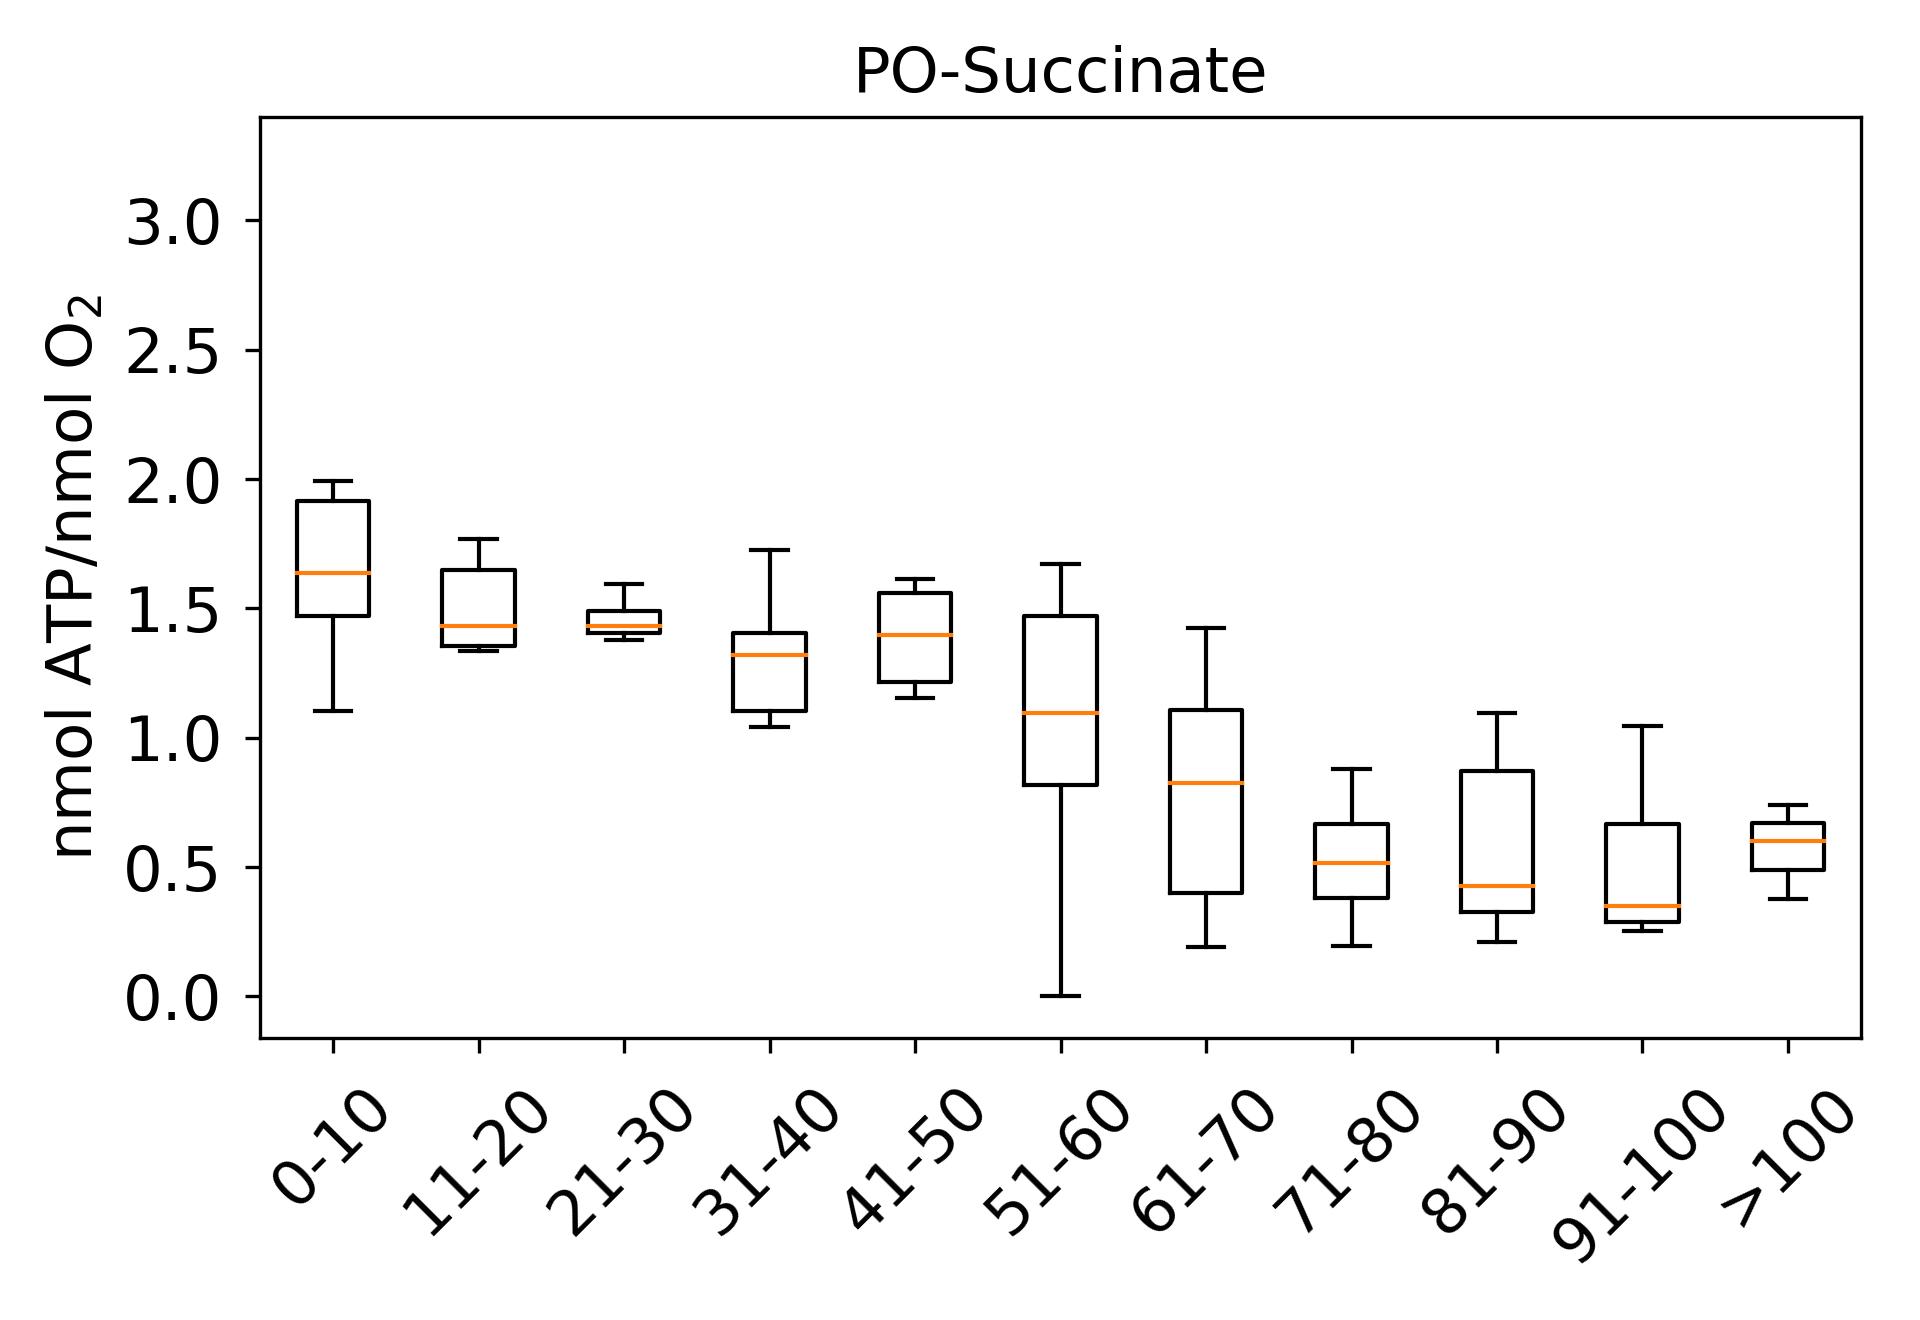
\includegraphics[width=0.33\textwidth]{part2/aging_boxplot_PO-Succinate.png}
		\label{fig:frassoni_boxplot_posucc}%
	}%
	\hfill%%%% ROW 3
	\subfloat[]{%
		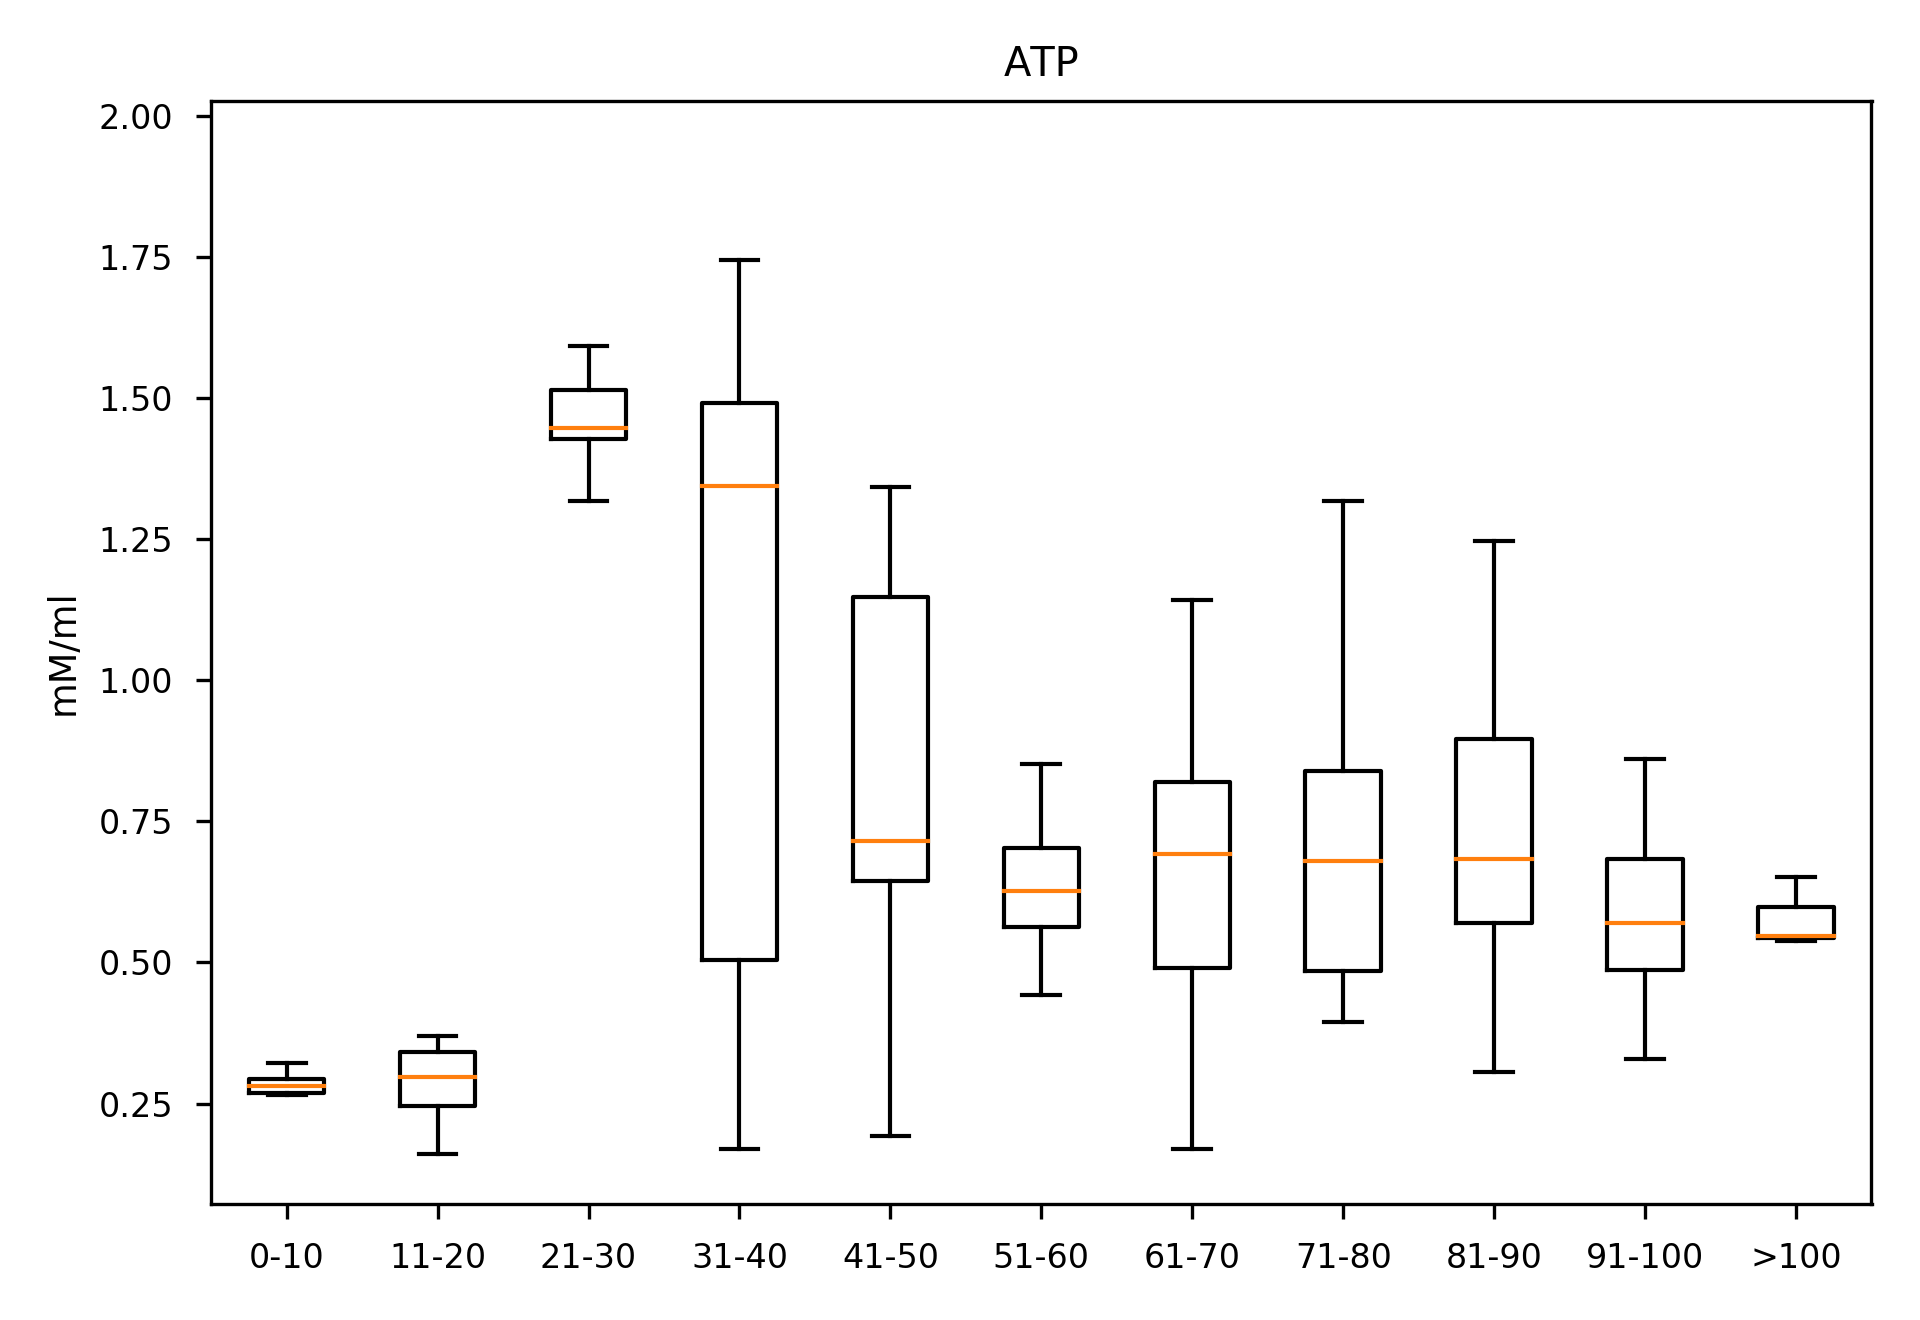
\includegraphics[width=0.33\textwidth]{part2/aging_boxplot_ATP.png}
		\label{fig:frassoni_boxplot_atp}%
	}%
	\subfloat[]{%
		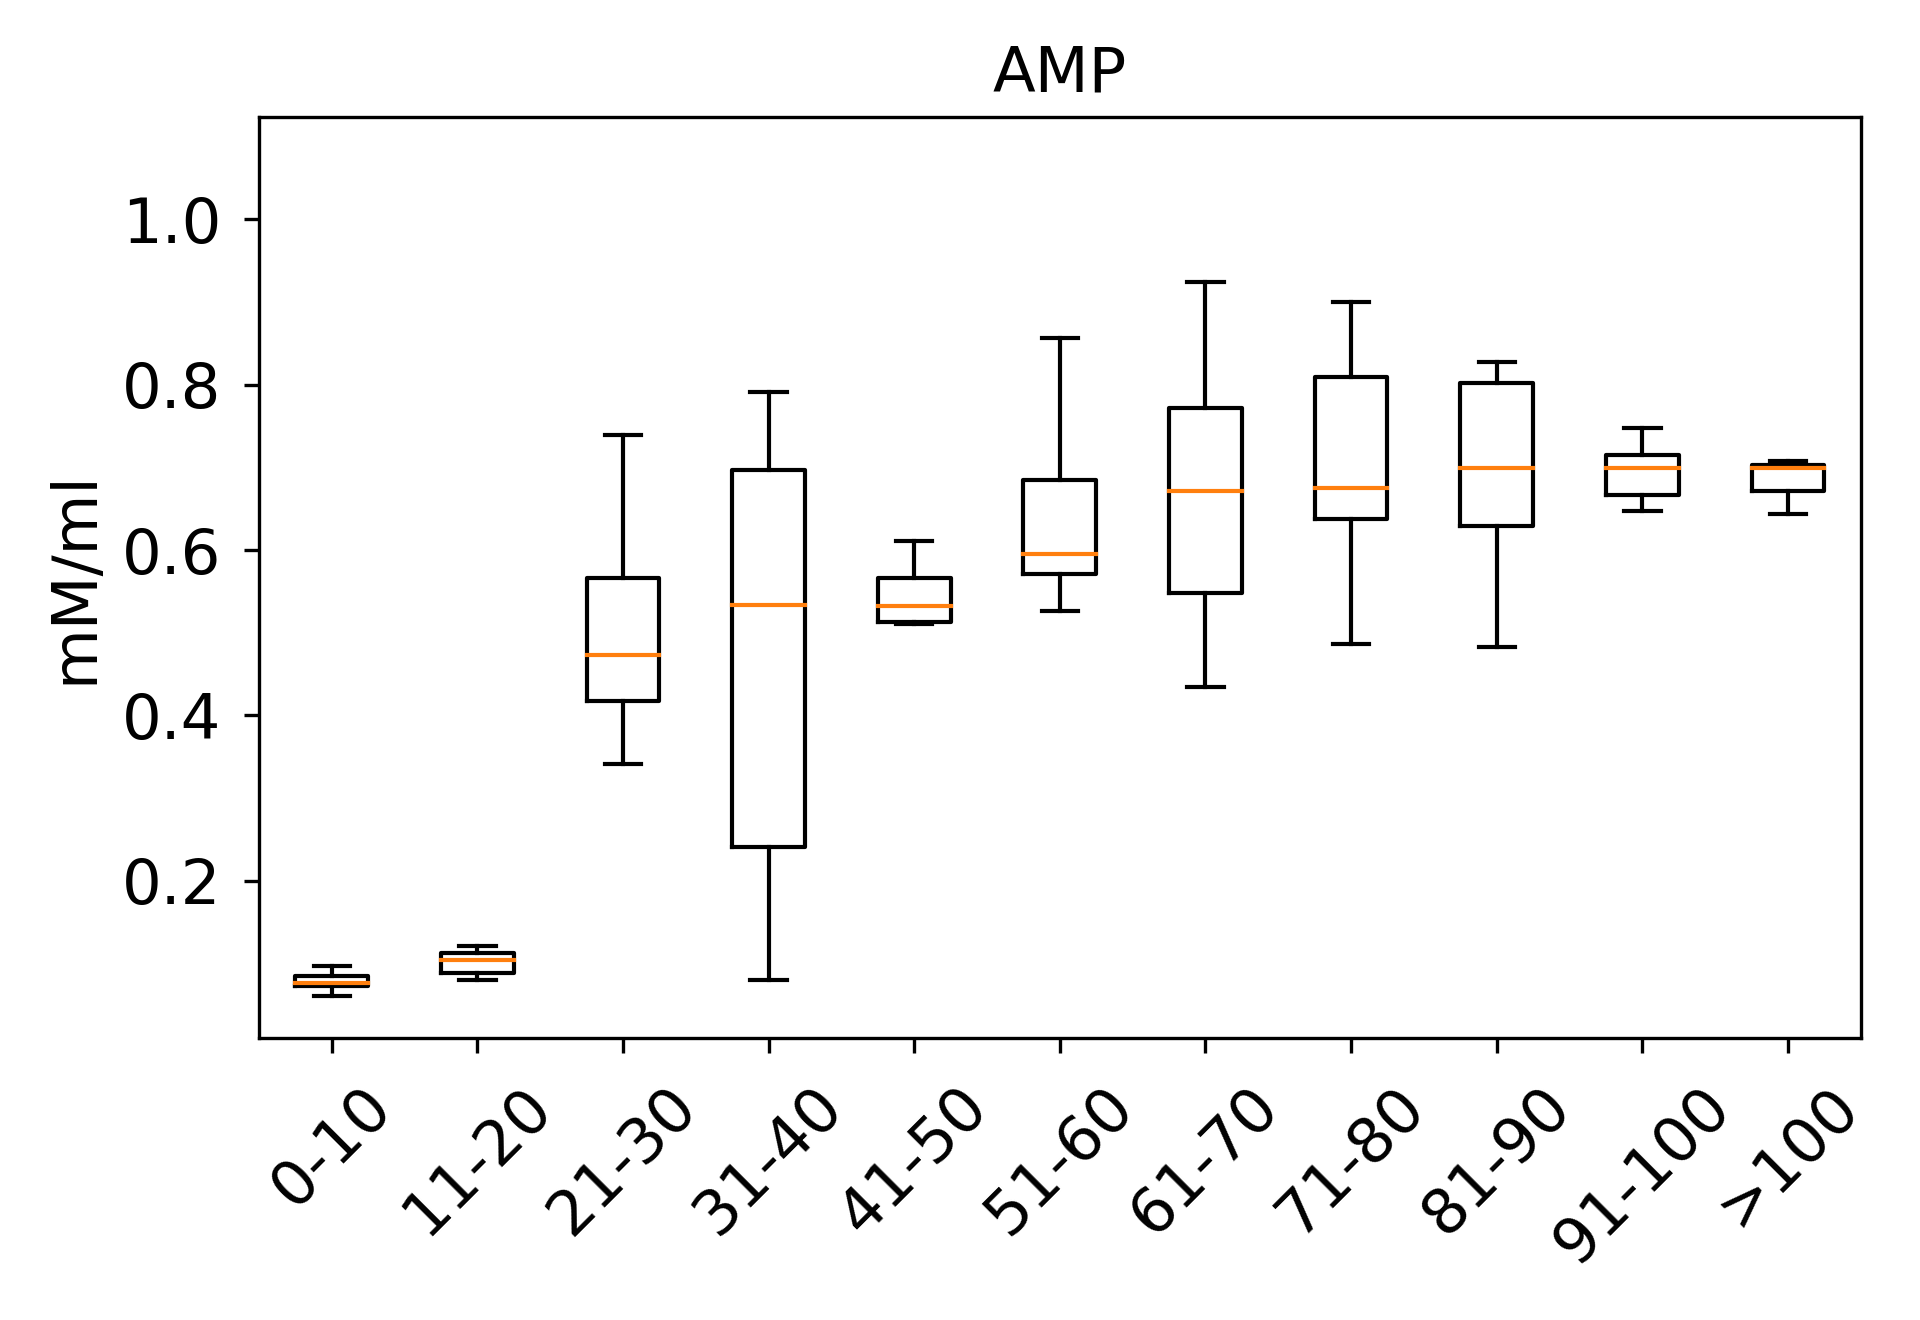
\includegraphics[width=0.33\textwidth]{part2/aging_boxplot_AMP.png}
		\label{fig:frassoni_boxplot_amp}%
	}%
	%	\hfill%
	\subfloat[]{%
		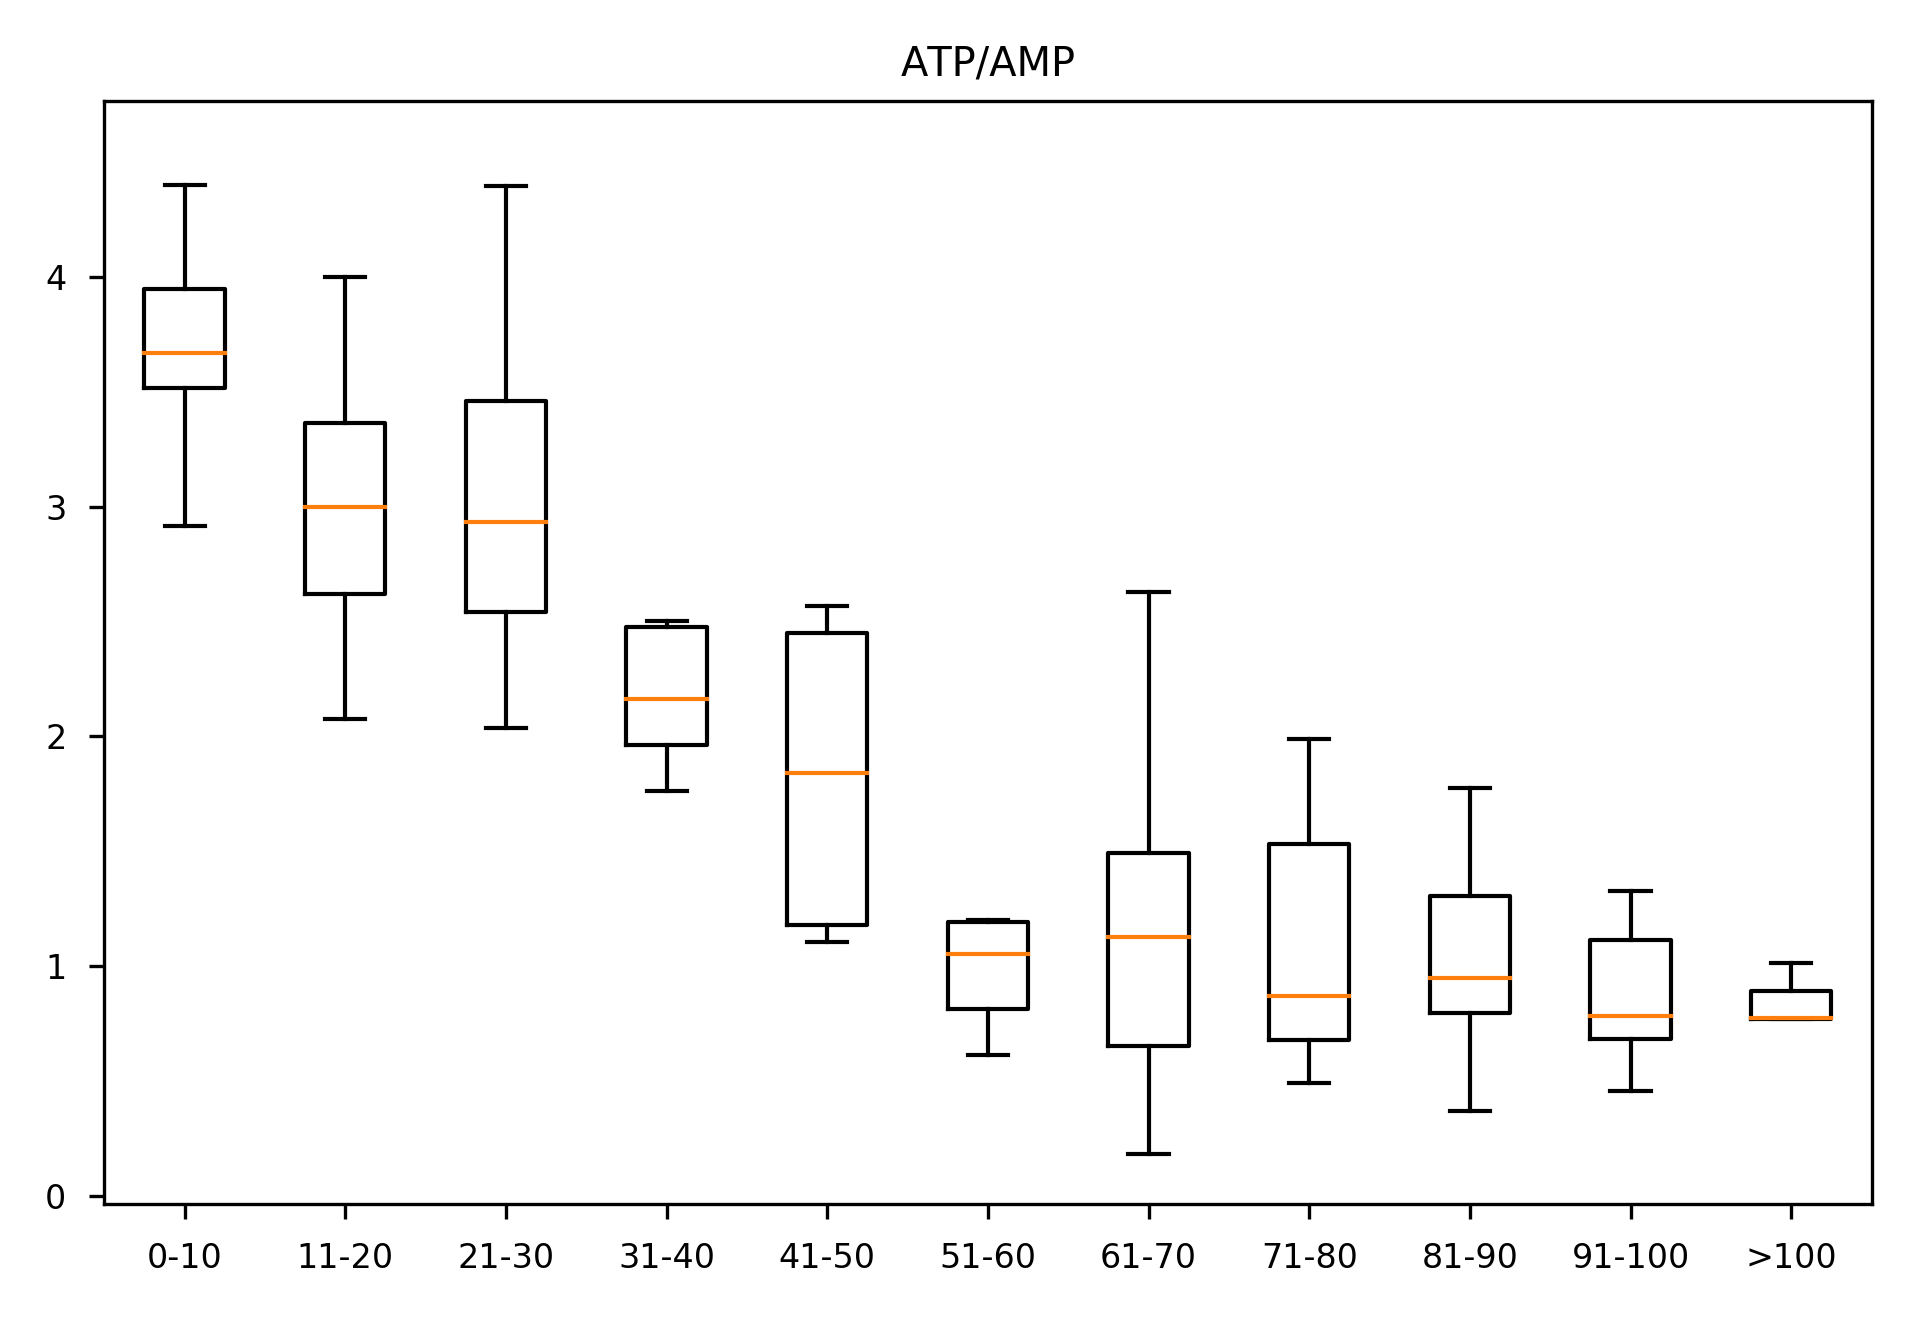
\includegraphics[width=0.33\textwidth]{part2/aging_boxplot_ATPAMP.png}
		\label{fig:frassoni_boxplot_atpamp}%
	}%
	\hfill%%%% ROW 4
	\subfloat[]{%
		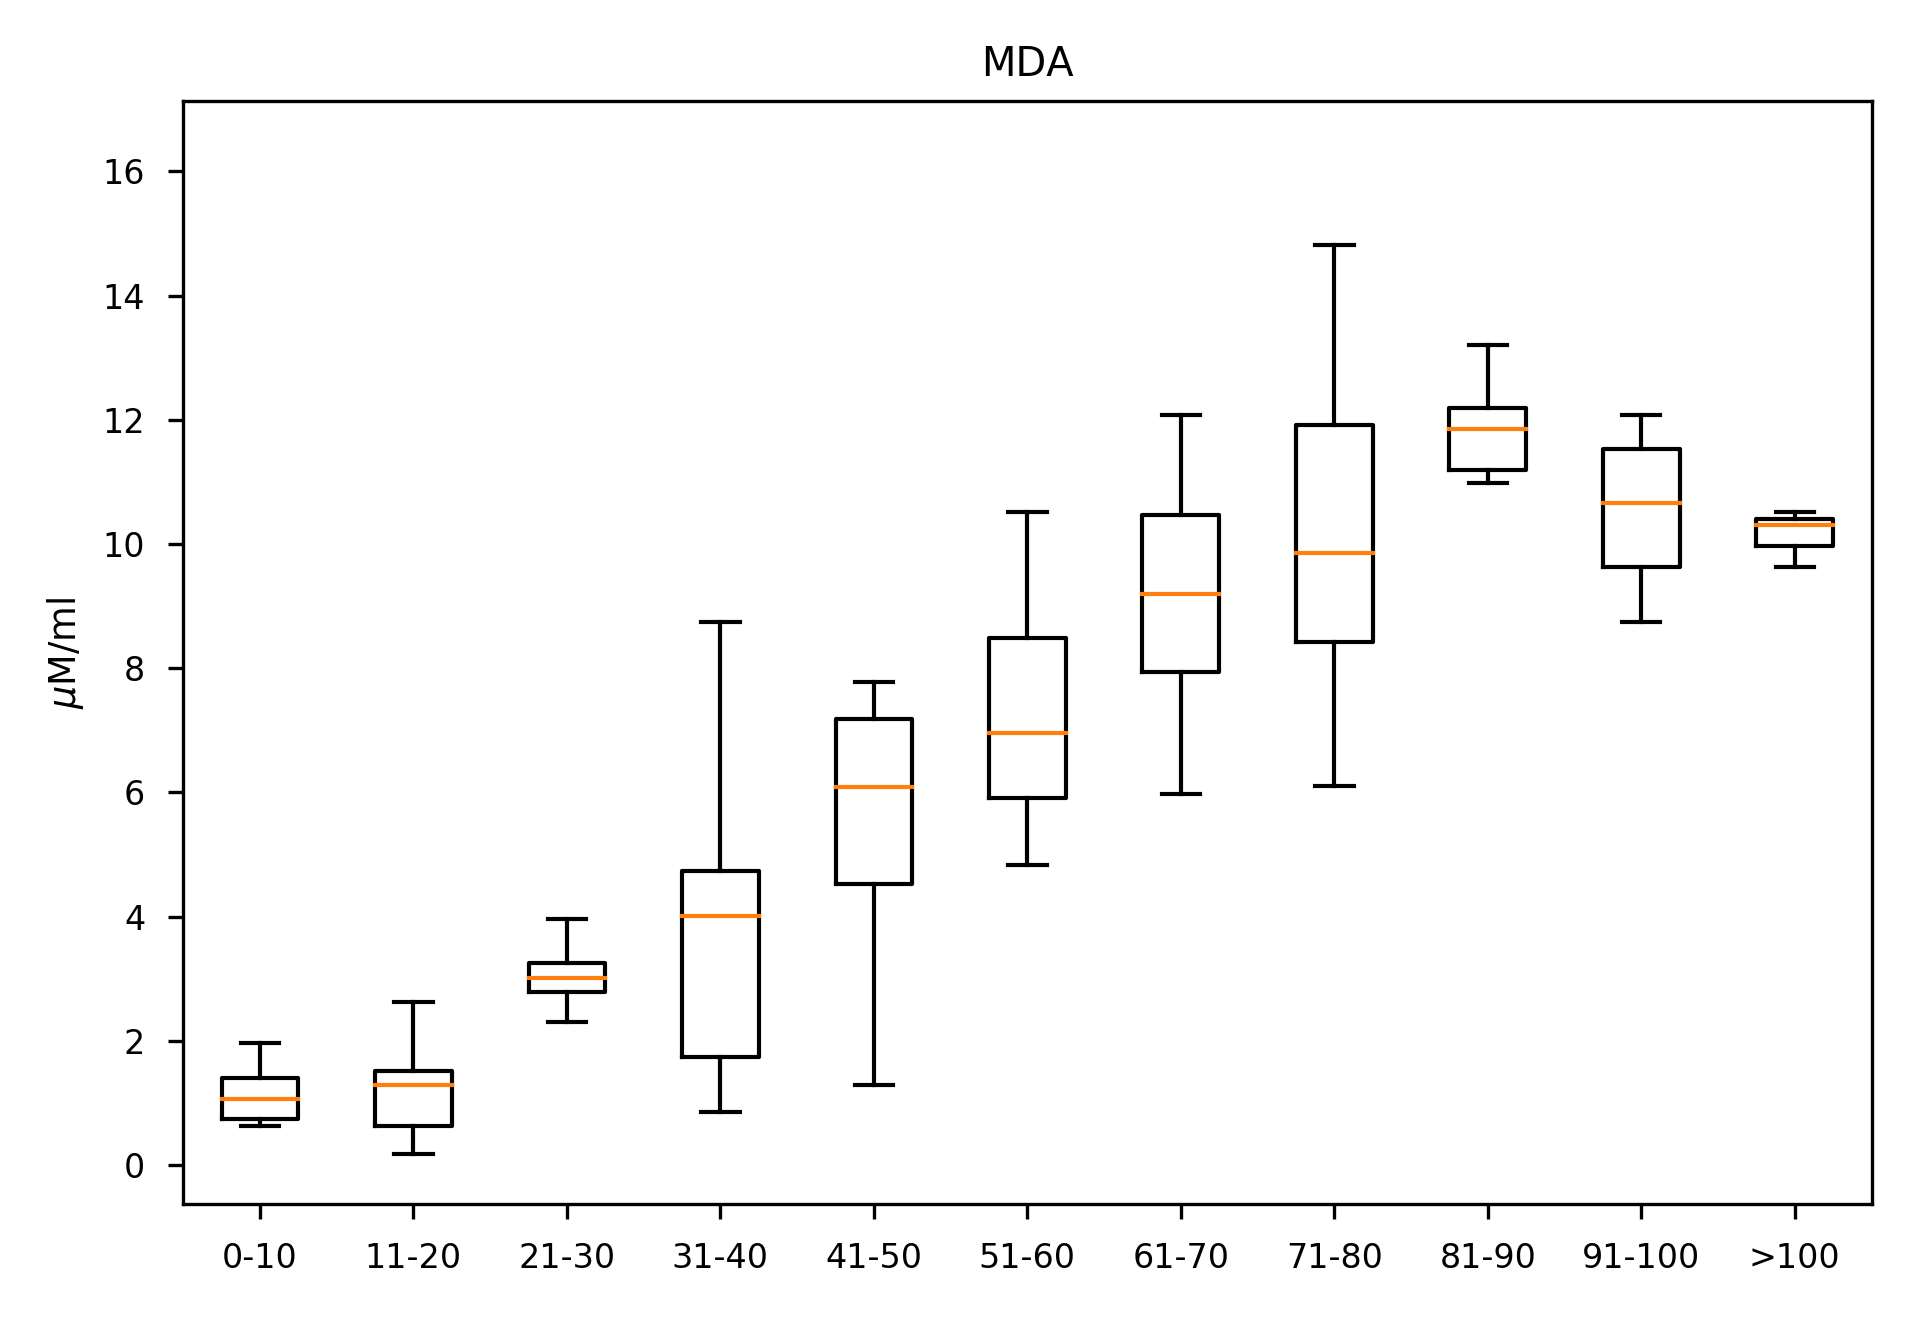
\includegraphics[width=0.33\textwidth]{part2/aging_boxplot_MDA.png}
		\label{fig:frassoni_boxplot_mda}%
	}%
	%	\hfill%
	\subfloat[]{%
		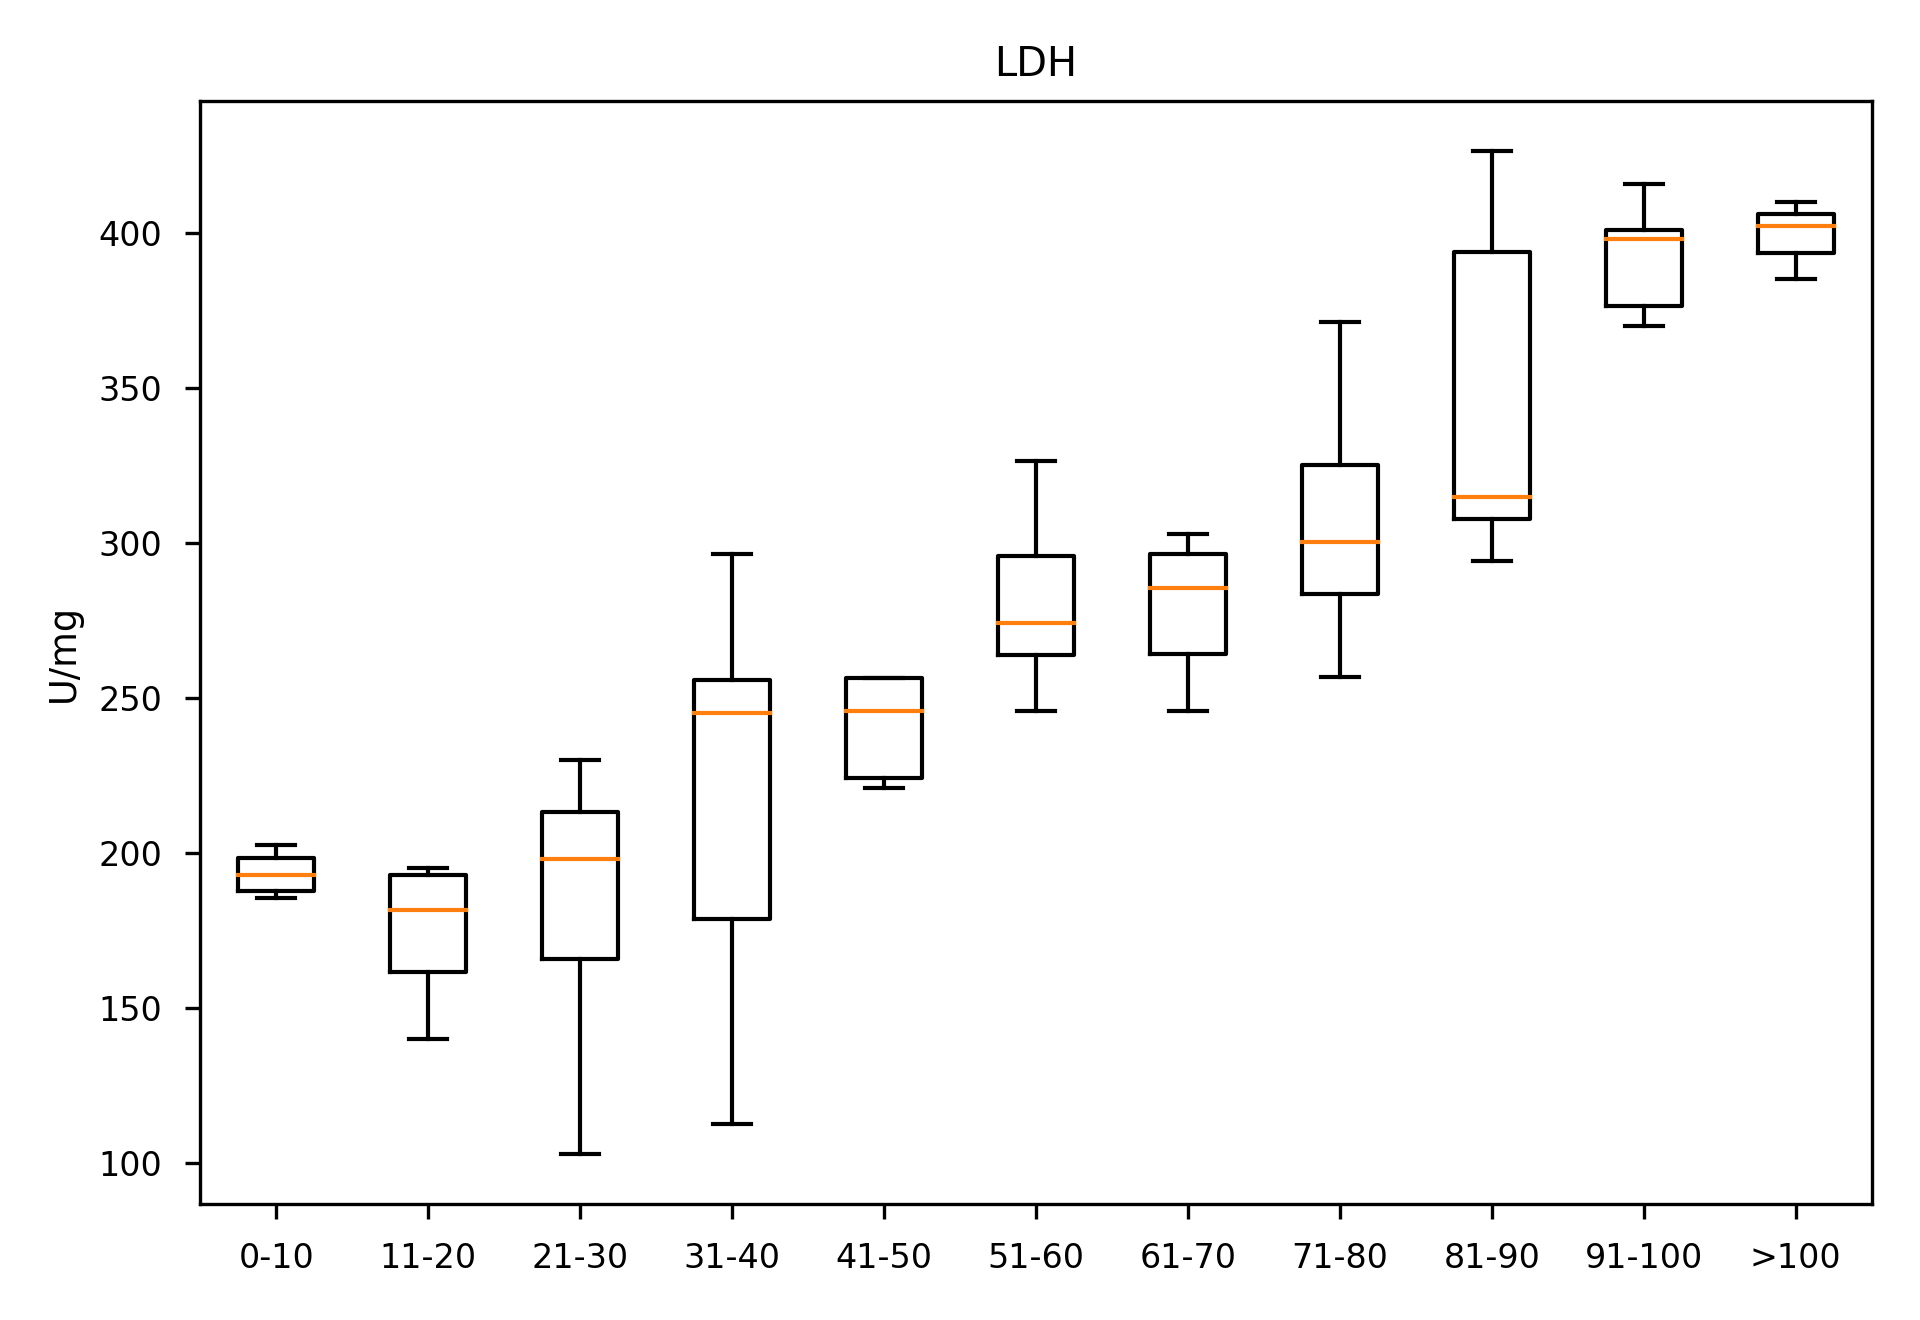
\includegraphics[width=0.33\textwidth]{part2/aging_boxplot_LDH.png}
		\label{fig:frassoni_boxplot_ldh}%
	}%
	\caption{Distribution of the collected molecular biomarker values grouped per decade.} \label{fig:frassoni_boxplot}
\end{figure}

So far, we have investigated on the relationship between the collected measures and the age of the individuals. Let's now focus on the relationship between the variables themselves. In order to investigate on possible collinearities in the data, we evaluated the Pearson correlation coefficient
\begin{equation}
	\rho(a, b) = \frac{\sum_{i=1}^n (a_i - \bar a)(b_i - \bar b)}{\sqrt{\sum_{i=1}^n(a_i-\bar a)^2 \sum_{i=1}^n(b_i-\bar b)^2}}
\end{equation}
(where $\bar c = \frac{1}{n}\sum_{i=1} c_i$ is the empirical mean of the variable $c$) for each pair of variables. This results in a symmetric $11 \times 11$ correlation matrix.
%In order to evaluate a specific age fingerprint,
We split the data in $5$ groups, one for each two-decades, and we represent the collinearity in each group with a symmetric heatmap in which dark red cells are associated with strong positive correlation, white cells represent no correlation and dark blue cells correspond to strong negative correlation, see Figure~\ref{fig:heatmaps}.
Thanks to this visualization, we can see that \atpamp and \popyrmal have positive correlation until the $6^{\text{th}}$ decade, while showing a negative correlation for elderly.
This suggests that up to approximately $60$ years, most of the cellular energy is produced by the mitochondria, while in older subjects this contribution decreases. The same observation can be made for \atpamp and \posucc, although in this case it is less evident. On the other hand, the correlation between \atpamp and \mda or \ldh activity is negative in young subjects, while flipping it sign after approximately $60$ years.
This is in line with the cellular need to increase the anaerobic metabolism that compensates the inefficiency of aerobic metabolism and the increment of oxidative stress which usually occurs for elderly.

\begin{figure}[]
	\centering
	\subfloat[]{%
		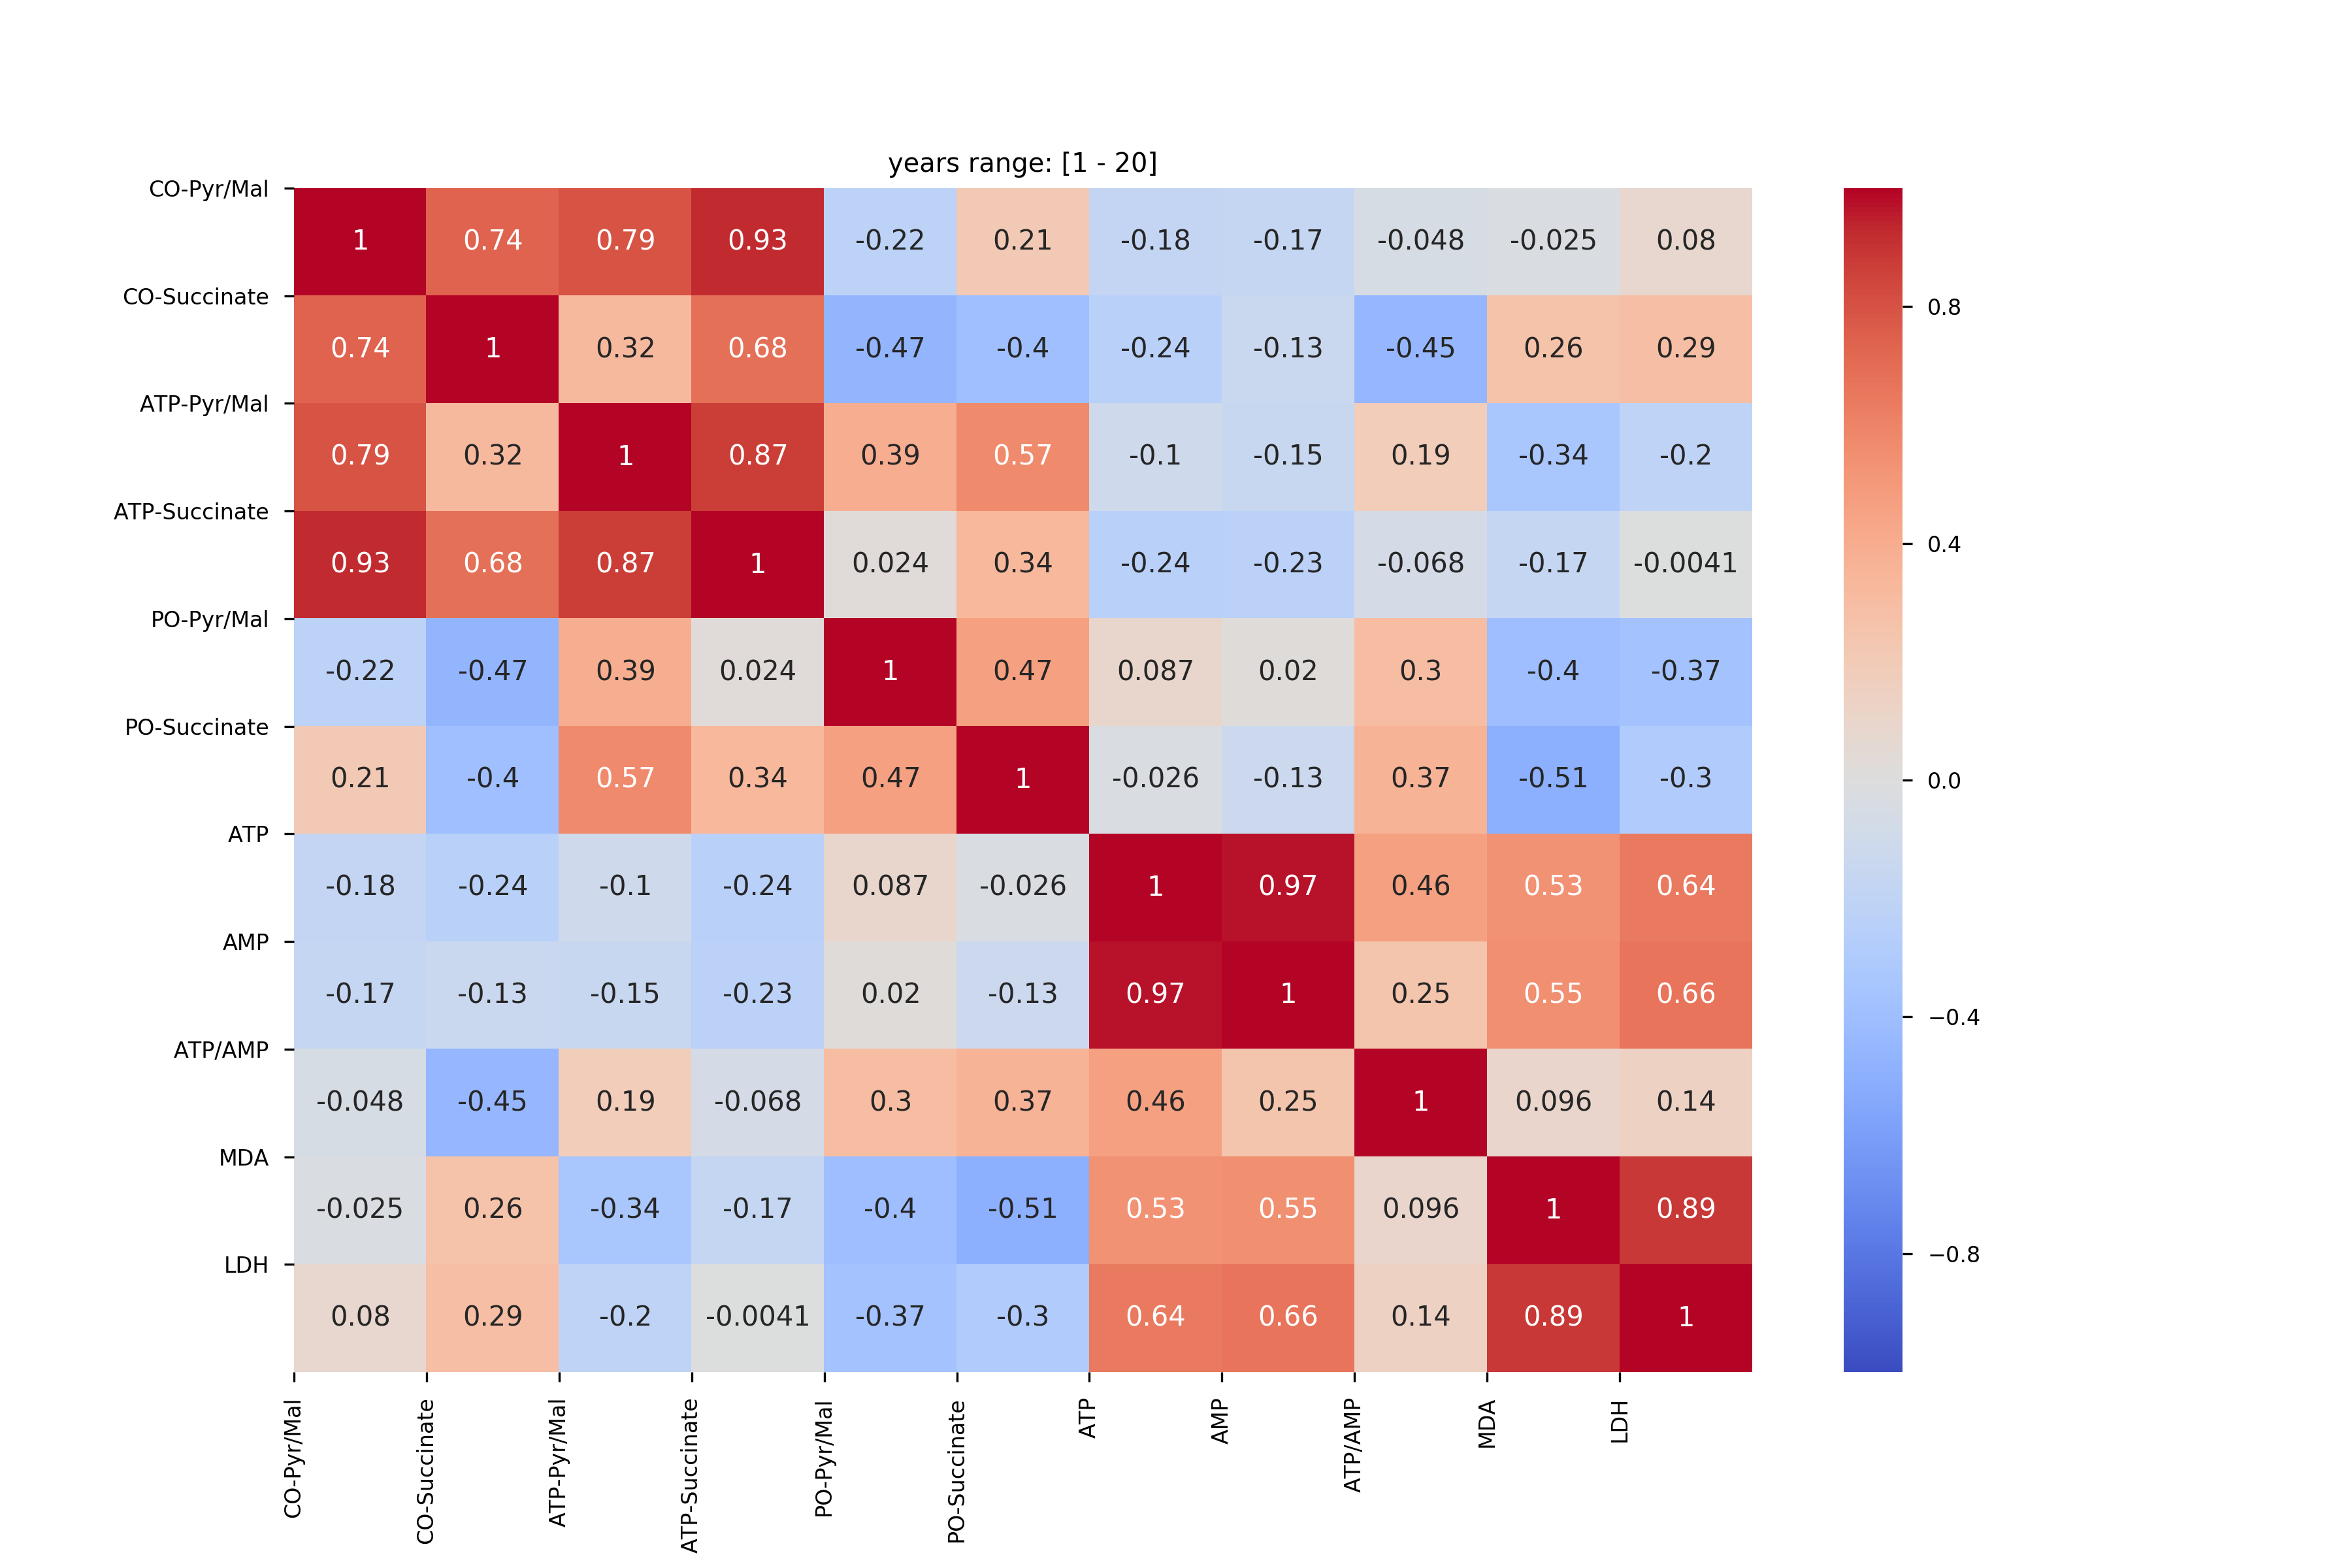
\includegraphics[width=0.5\textwidth]{part2/aging_heatmap_years range_0.png}
		\label{fig:heatmaps1}%
	}%
	\subfloat[]{%
		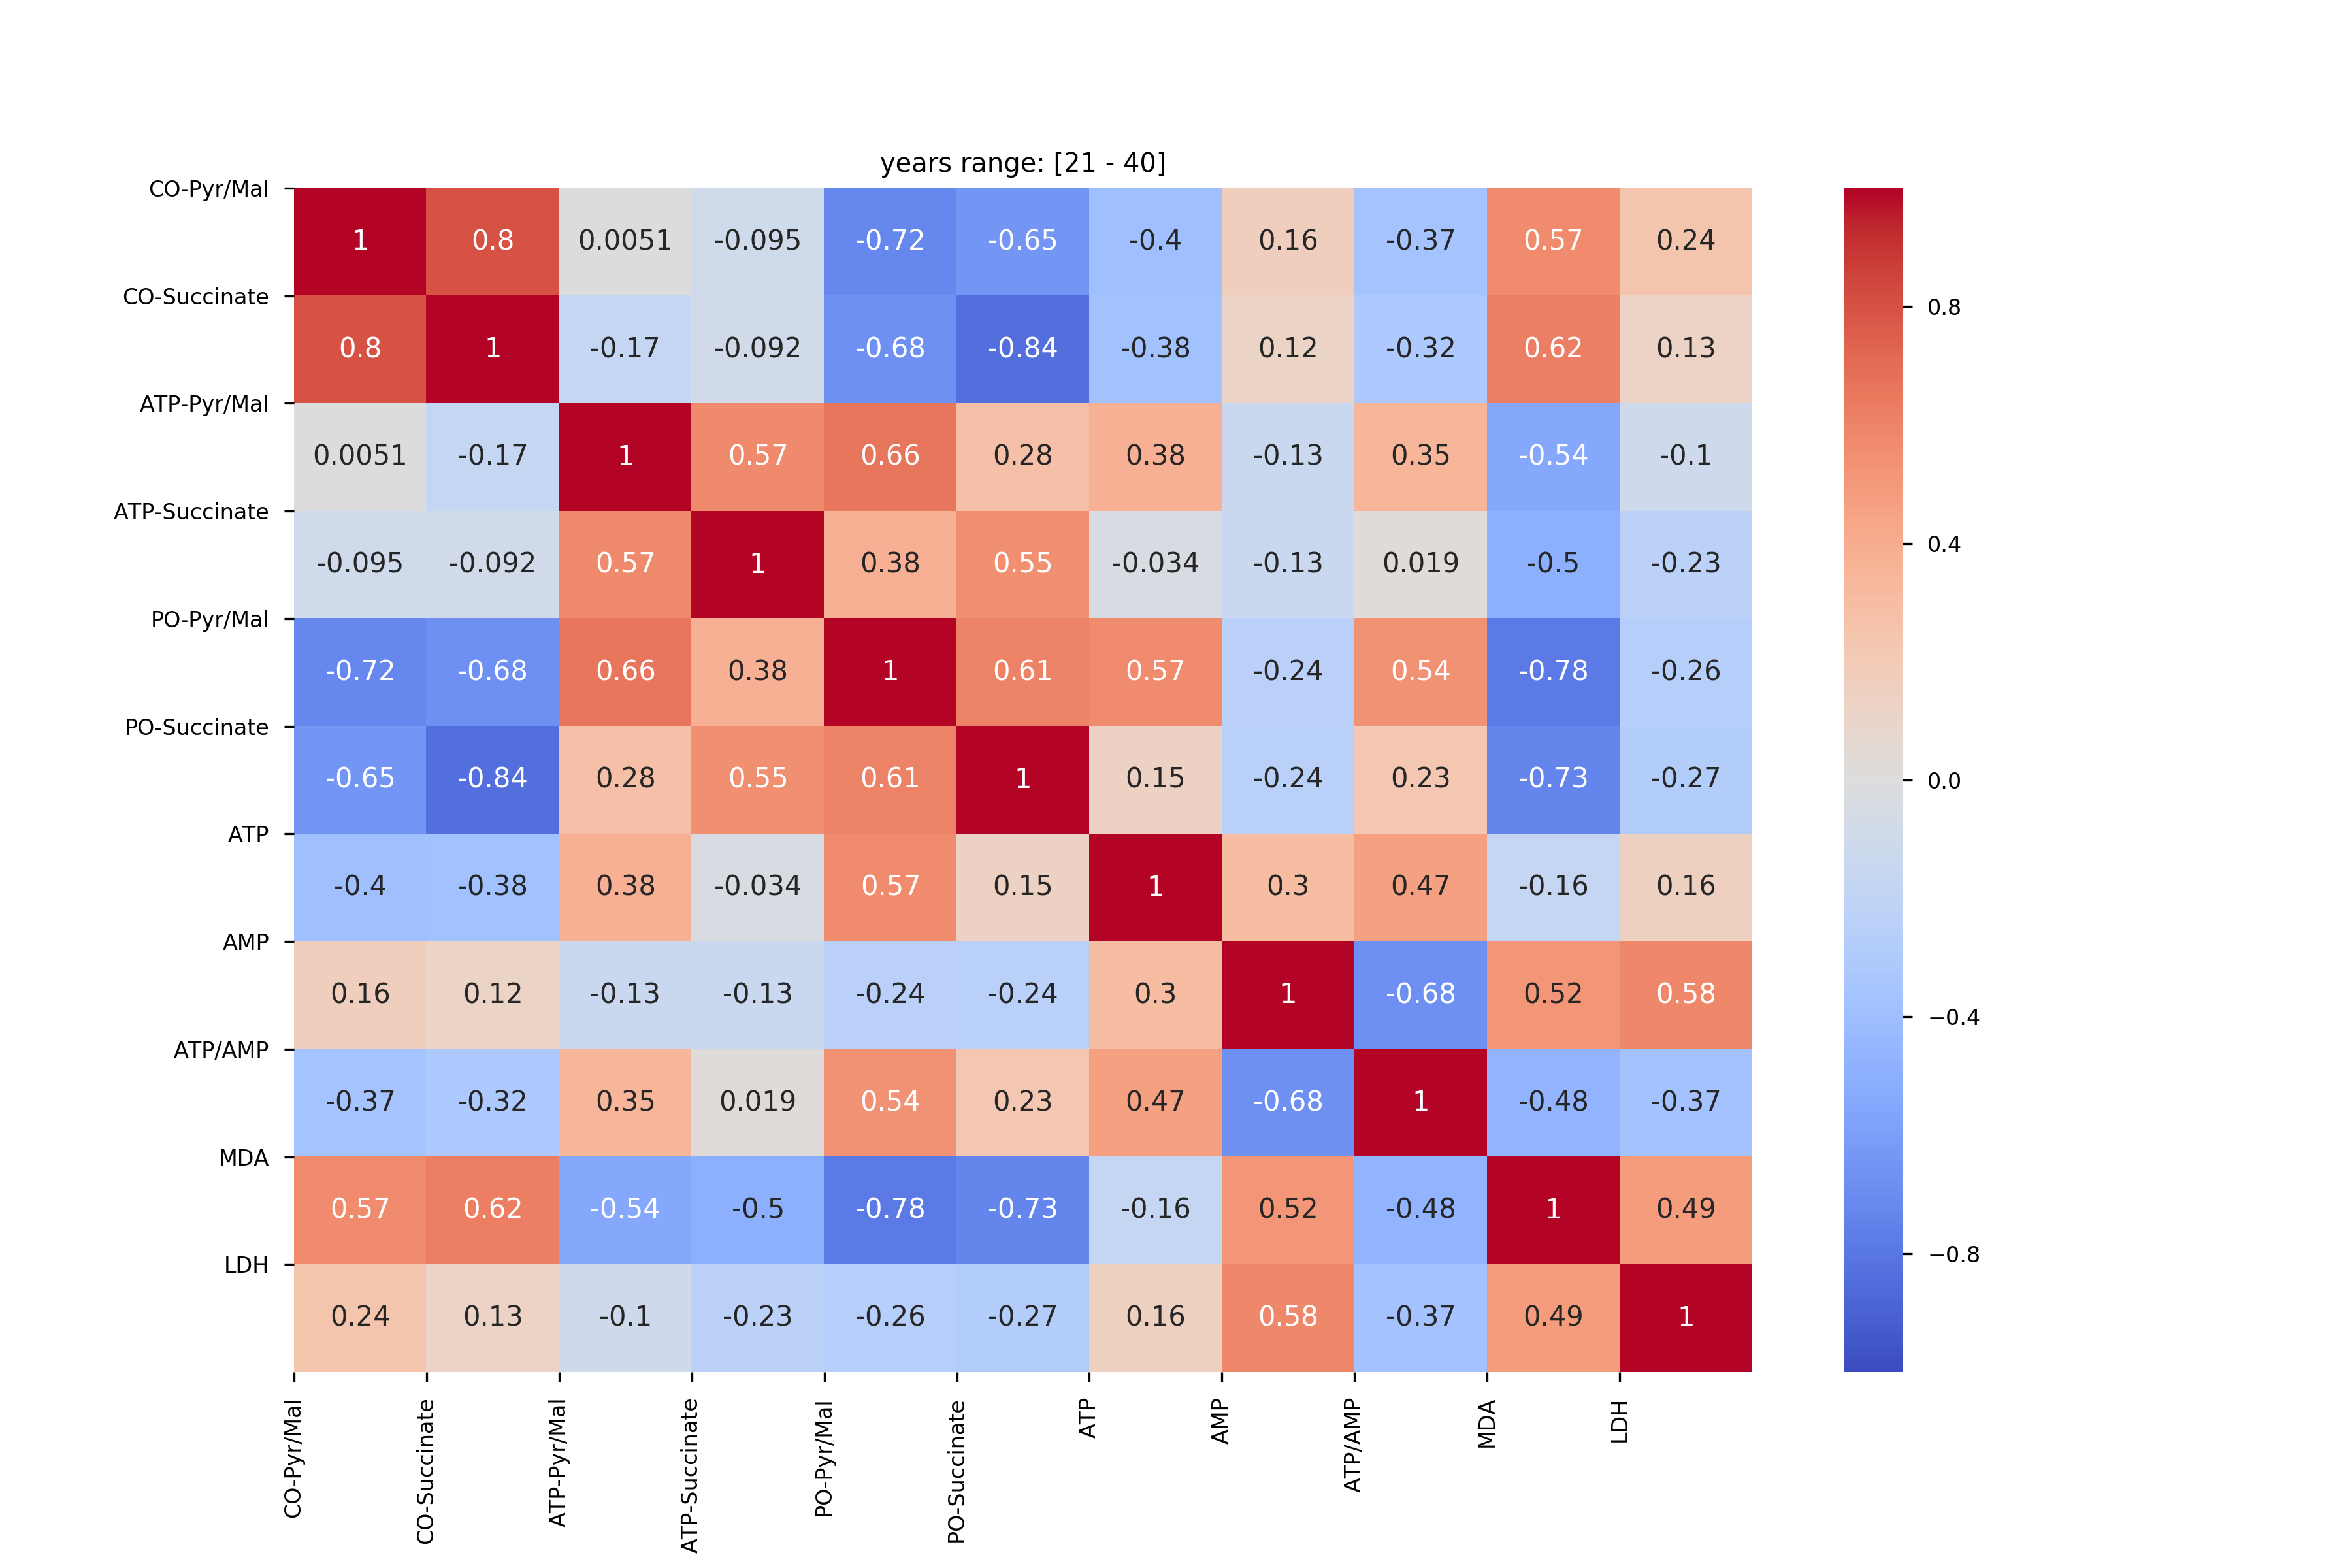
\includegraphics[width=0.5\textwidth]{part2/aging_heatmap_years range_1.png}
		\label{fig:heatmaps2}%
	}%
		\hfill%
	\subfloat[]{%
		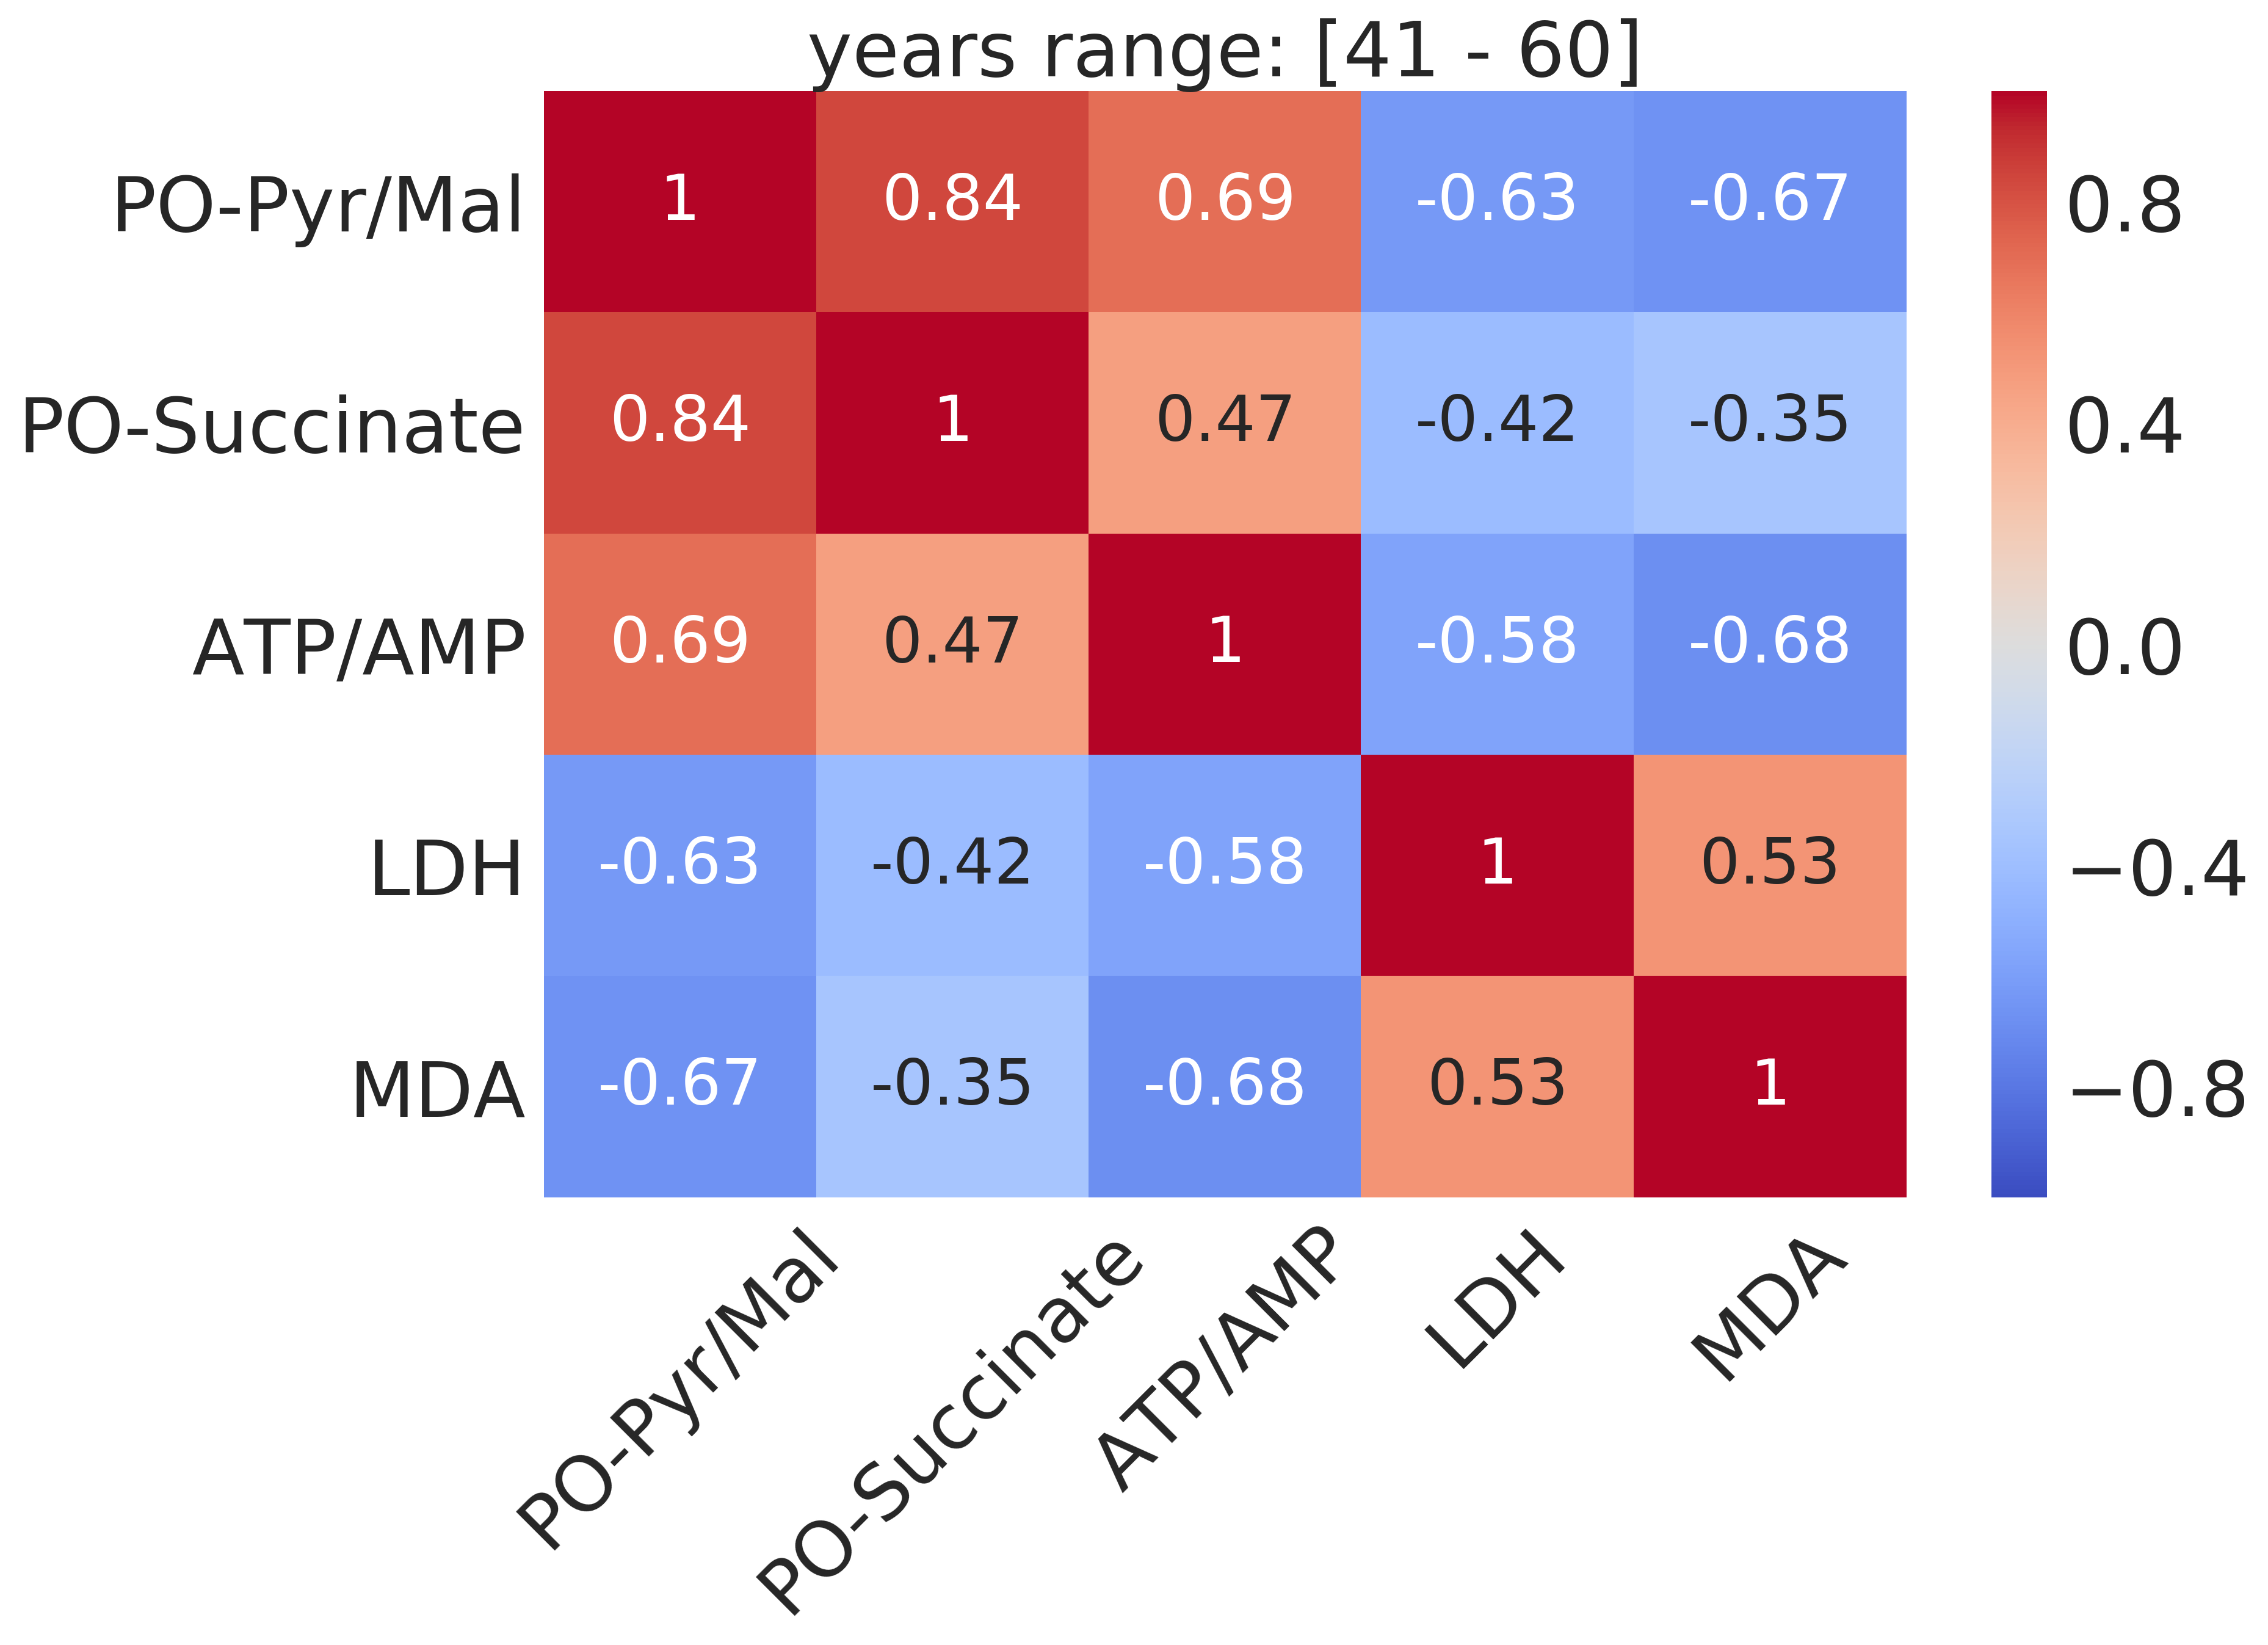
\includegraphics[width=0.5\textwidth]{part2/aging_heatmap_years range_2.png}
		\label{fig:heatmaps3}%
	}%
%	\hfill% %%%% 
	\subfloat[]{%
		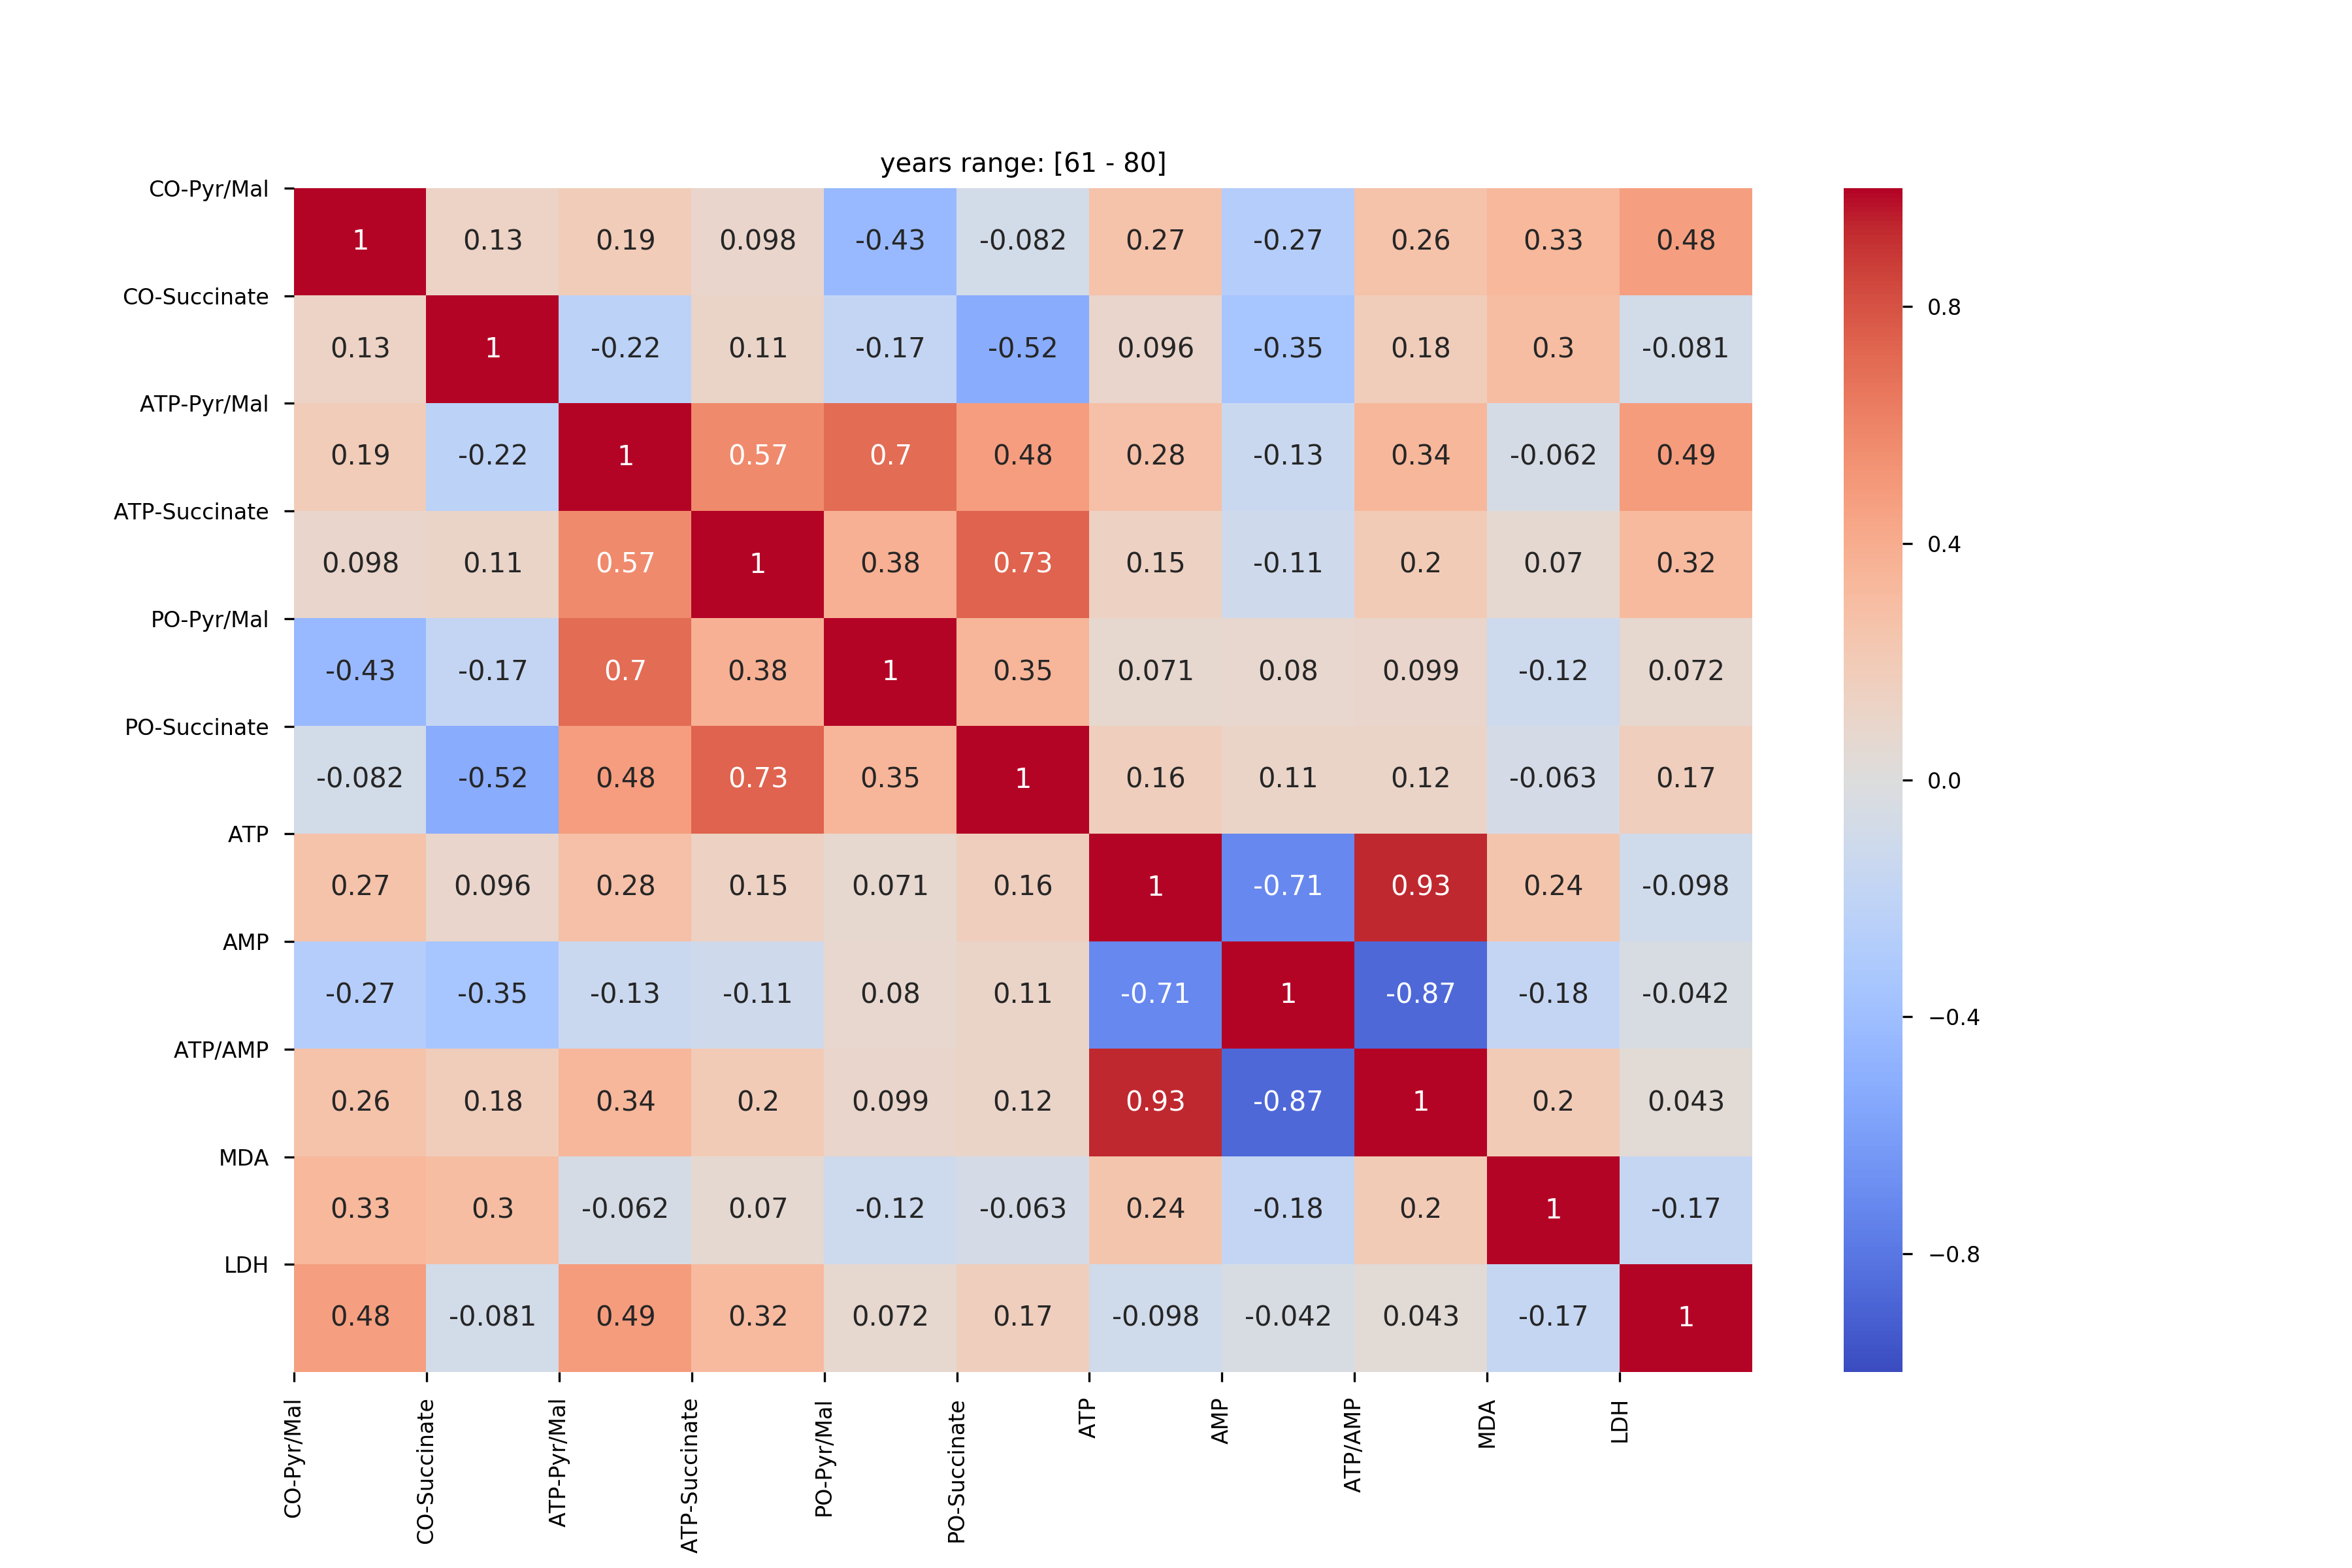
\includegraphics[width=0.5\textwidth]{part2/aging_heatmap_years range_3.png}
		\label{fig:heatmaps4}%
	}%
   \hfill
	\subfloat[]{%
		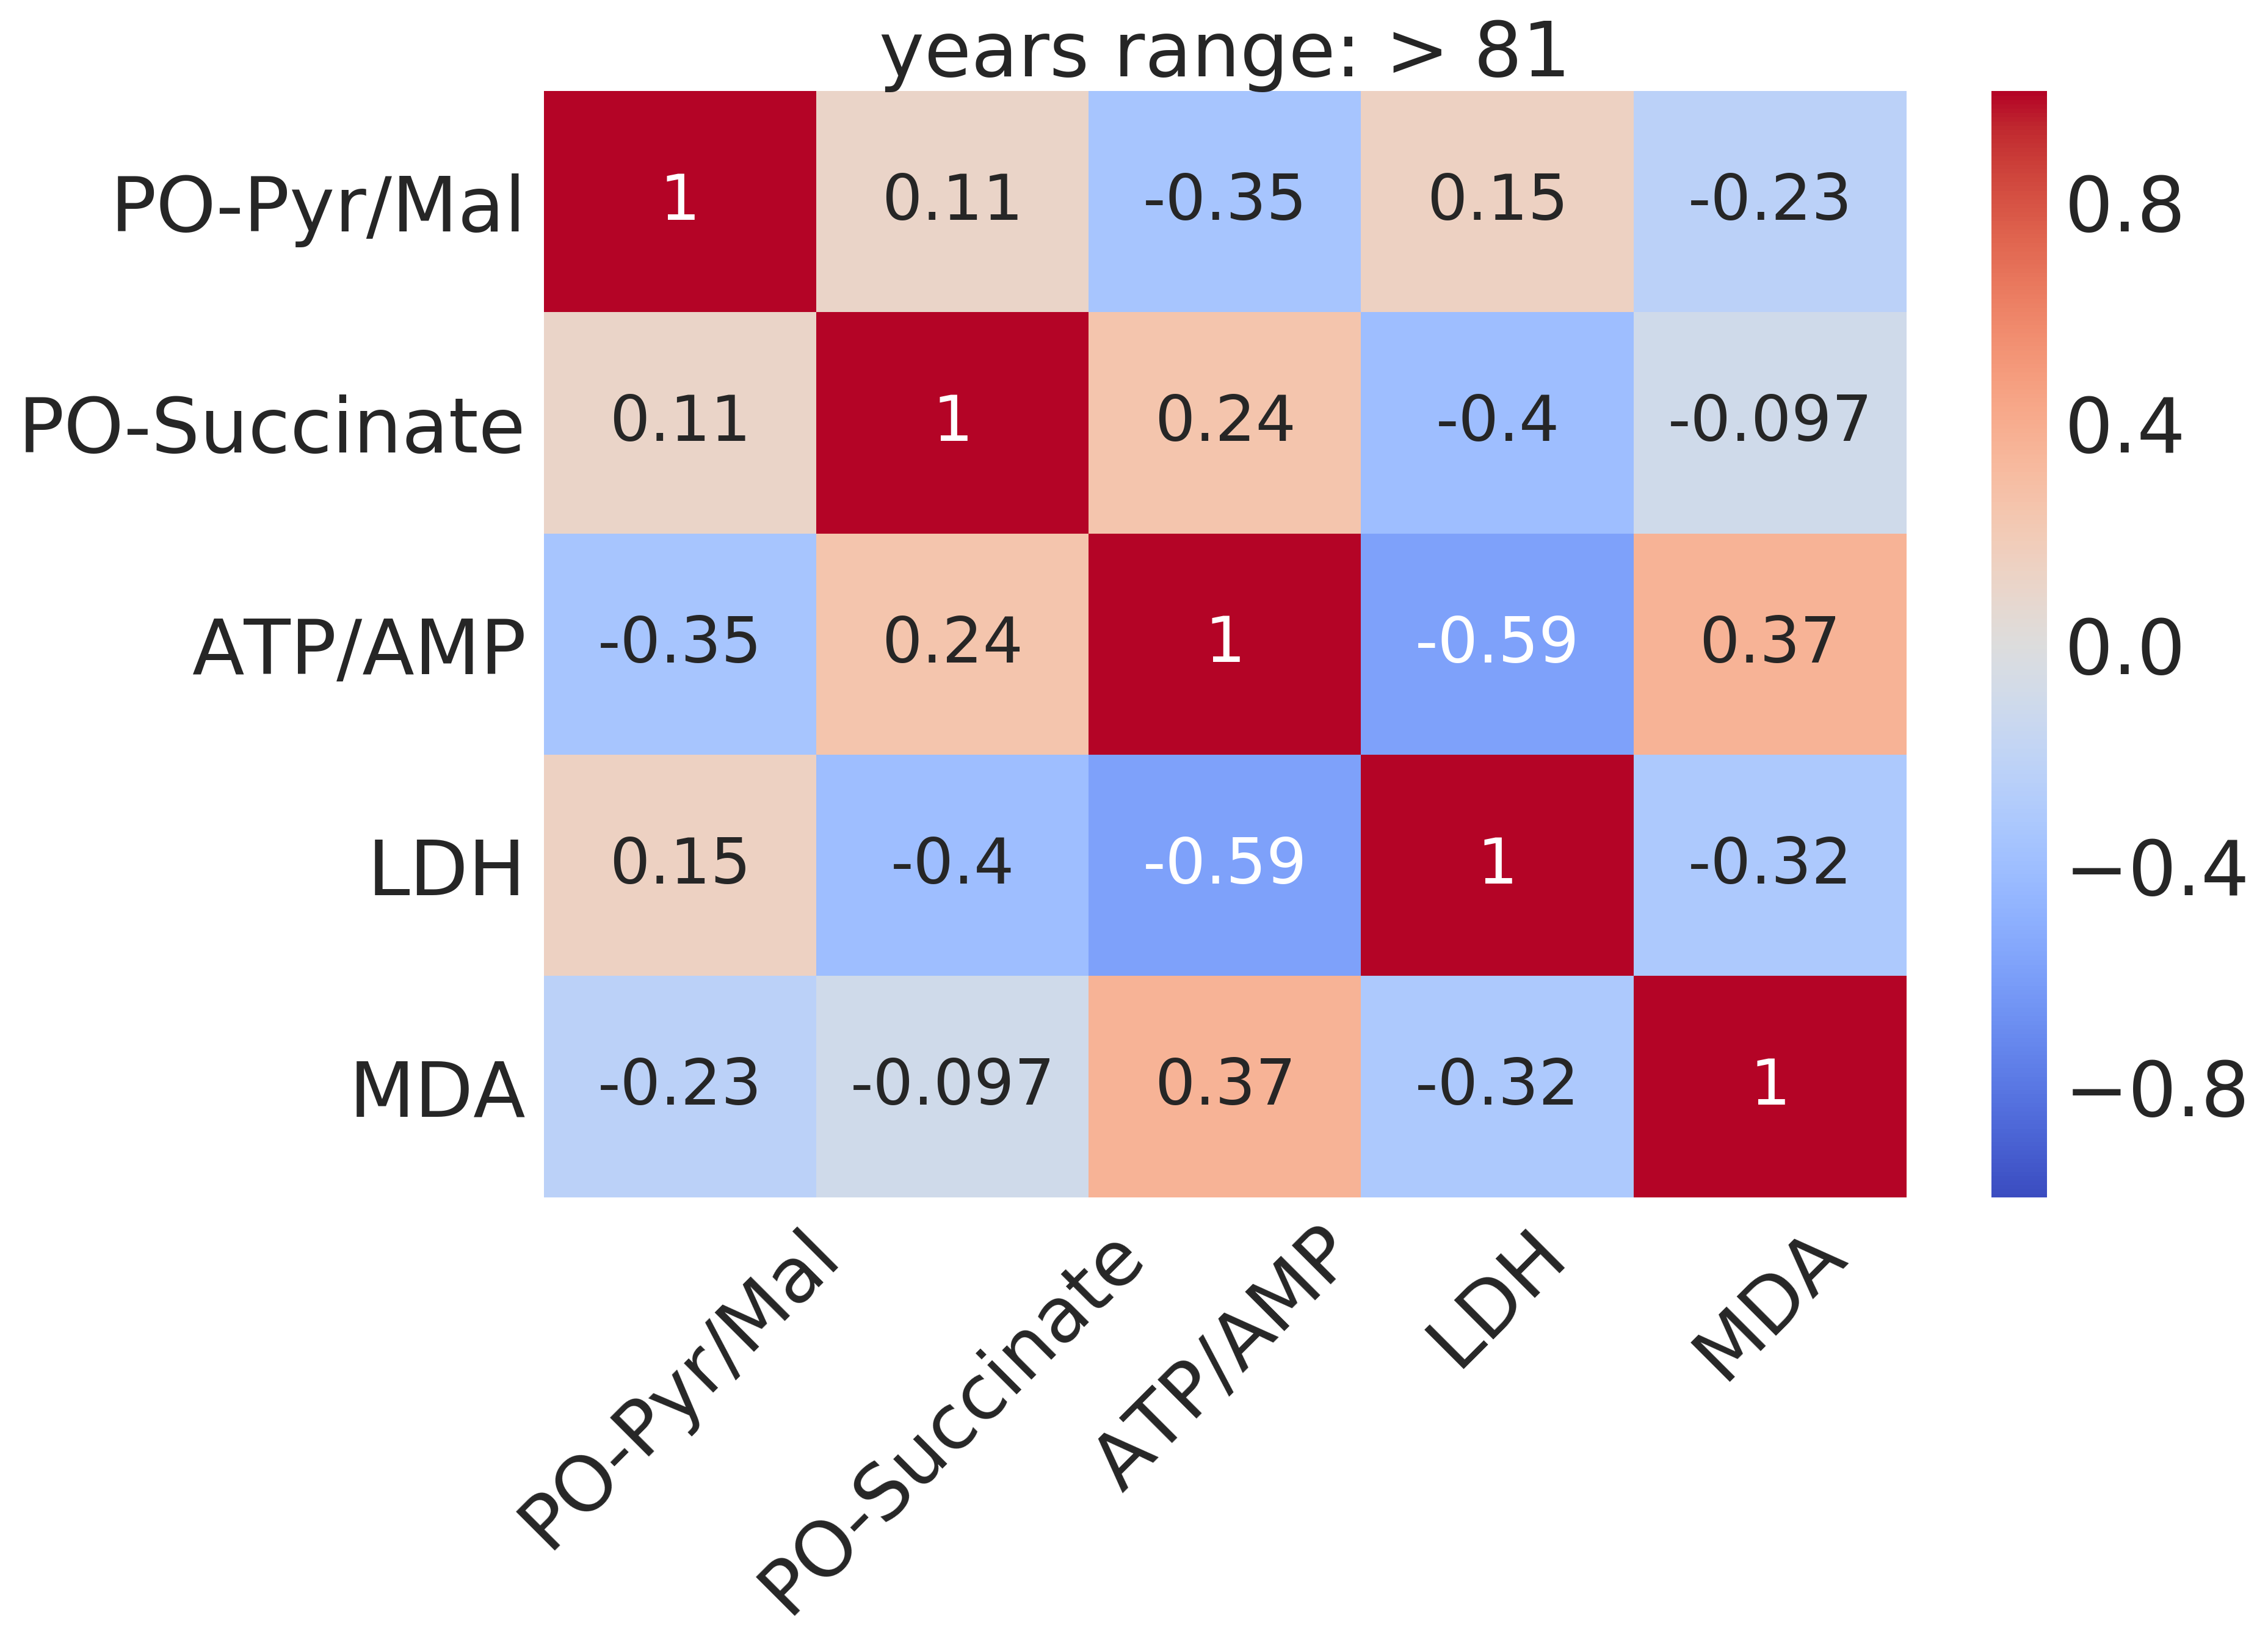
\includegraphics[width=0.5\textwidth]{part2/aging_heatmap_years range_4.png}
		\label{fig:heatmaps5}%
	}%
	\caption{The $11 \times 11$ symmetric heatmaps representing the Pearson correlation coefficient of the collected variables in the $5$ age groups: $[1-20]$ (a), $[21-40]$ (b), $[41-60]$ (c), $[61-80]$ (d), $>81$ (e).} \label{fig:heatmaps}
\end{figure}


Let's now try to visualize the collected data in a scatter plot. In order to do that, we shall first reduce the dimensionality of the problem, as described in Section~\ref{sec:dimred}.
Most of the variables showed strong linear correlation between themselves and some of them also with respect to the age. We then reduce the dimensionality of the problem following a two step pipeline:
\begin{enumerate*}[label=(\roman*)]
	\item data standardization followed by
	\item via linear PCA.
\end{enumerate*}
Our hope is to be able to recognize some, approximately linear, temporal structure. The resulting scatter plot is presented in Figure~\ref{fig:frassoni_PCA}.
Each point in the scatter plot represents a subject color coded according to the age.
Let's read the image from left to right.
As we can see, it looks like the subjects are partially grouped according to their age. In the top left corner of Figure~\ref{fig:frassoni_PCA} subjects with approximately $20$ years (or less) are clustered together. At the center bottom of the plot we can recognize individuals around their thirties. Then, following an approximately linear law from center bottom to top right we can see that the age increases until reaching the elderly, color coded in dark red.
The insightful data visualization in Figure~\ref{fig:frassoni_PCA}, gives us hopes to be able to devise a supervised strategy to predict the age of a given individual starting from these molecular biomarkers.

\begin{figure}[]
	\centering
	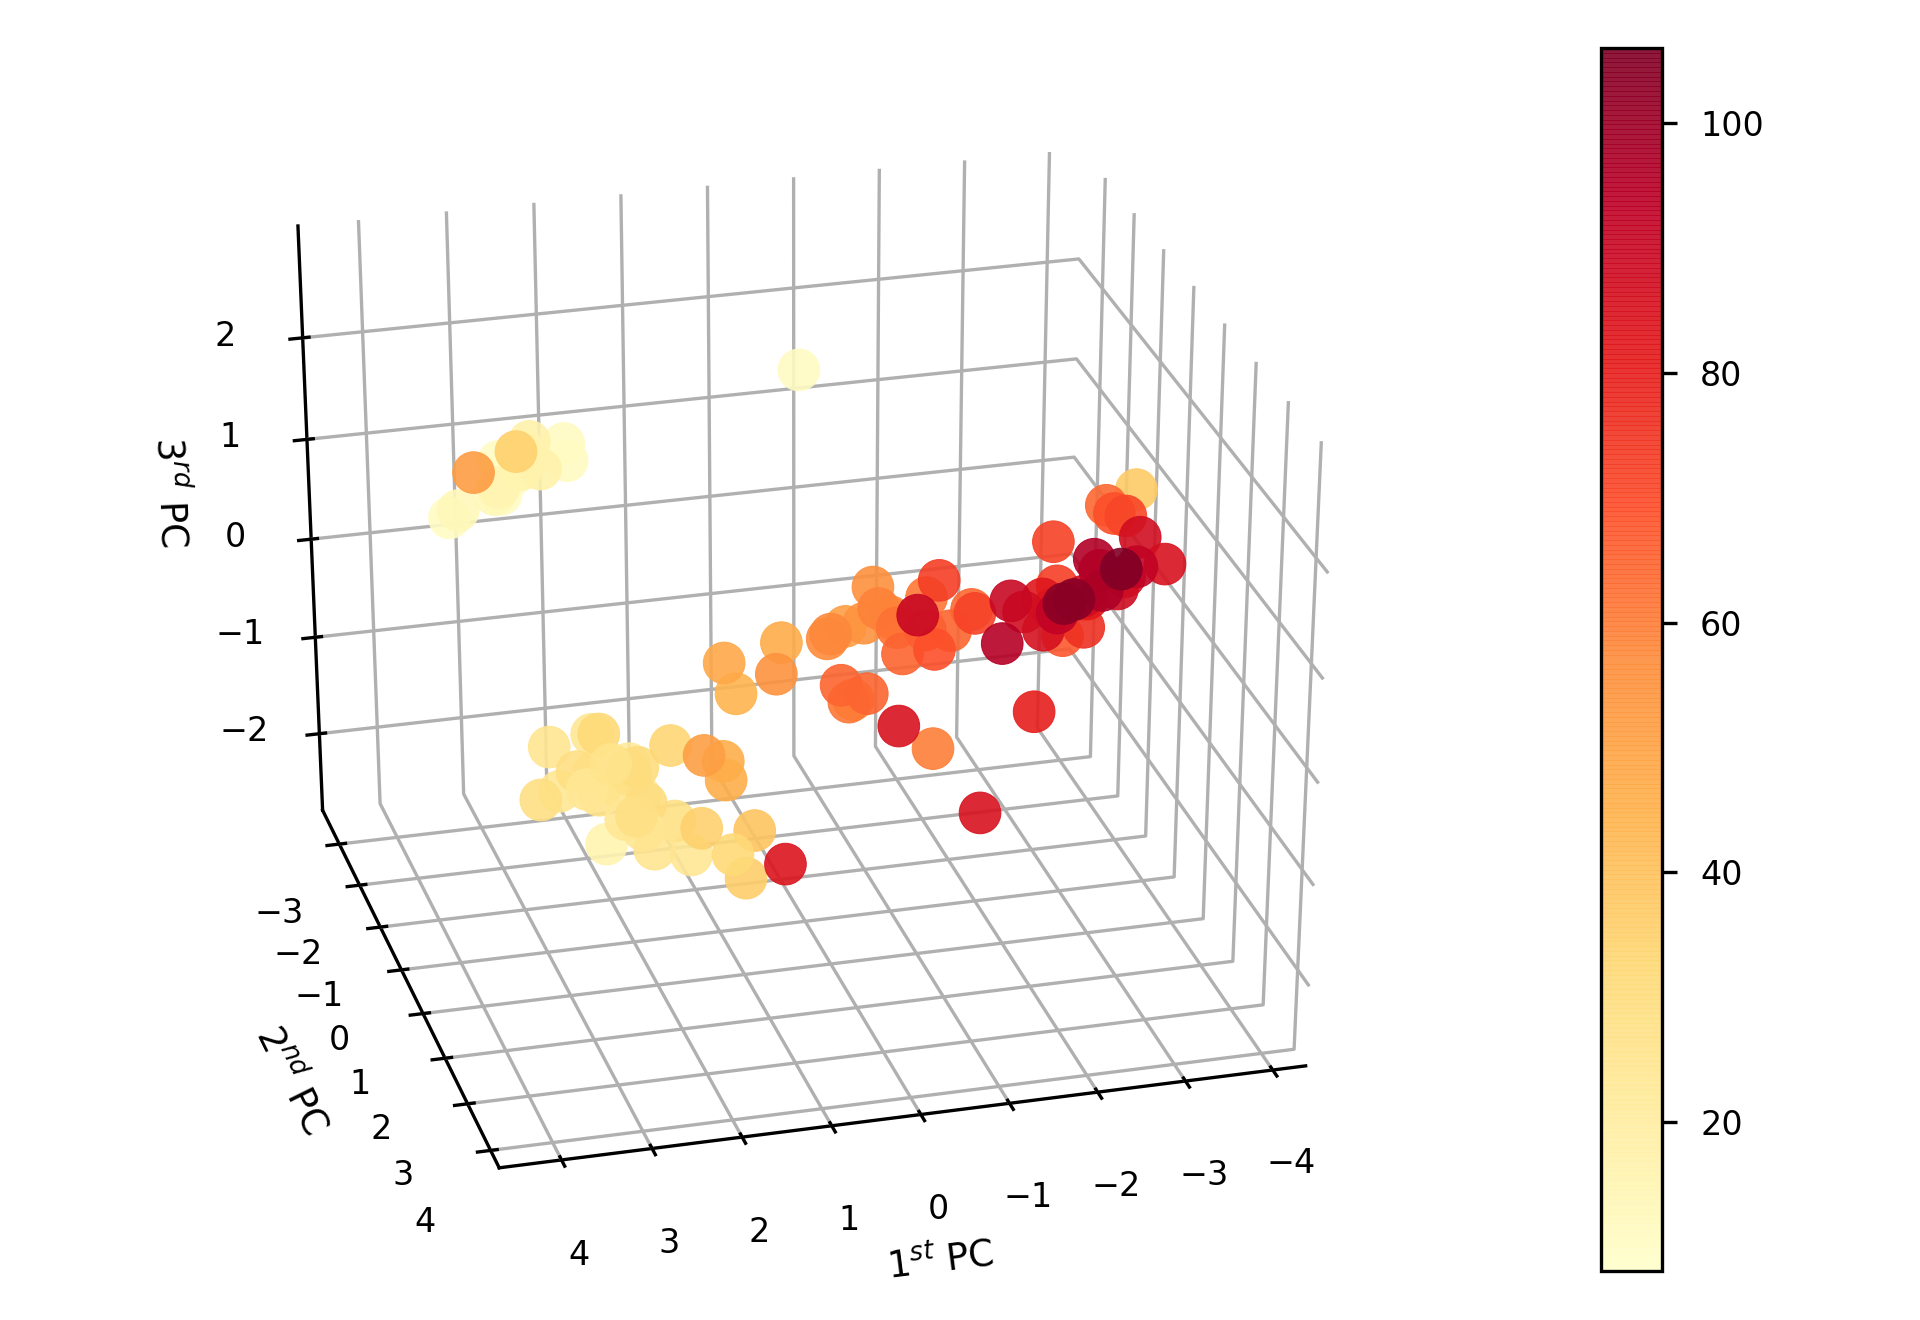
\includegraphics[width=0.8\textwidth]{part2/aging_PCA.png}
	\caption{Scatter plot obtained after projecting the data in a $3D$ space via linear PCA. The color-coding represents the age of the individuals.} \label{fig:frassoni_PCA}
\end{figure}


\section{Metabolic age prediction} \label{sec:frassoni_regression}
% pipeline + assessment + model challenge
This section presents the development of the regression model for the age prediction task presented in this chapter.

To this aim, we imputed the small fraction of missing values following the $k$-nearest neighbors (with $k=3$) proposed in~\cite{troyanskaya2001missing}. So, the development of the predictive model can take advantage of the total number of individuals ($n=118$).

In the EDA we realized that most of the input variables show a quasi-linear relationship with the age. Moreover, we also realized that most of the input variables have a strong pairwise linear correlation. Therefore it seems sensible to investigate whether a polynomial feature expansion could be beneficial for the age prediction.
To this aim, we devised the following experimental setting.

A cross-validated estimate of four popular regression scores: $\text{R}^2$, MAE, MSE and EV (defined in Section~\ref{sec:performance_metrics}) is evaluated.
In order to achieve a better estimate of the empirical distribution of such scores, we opted for a Monte Carlo cross-validation strategy.
%\todo{should have been stratified -> correggere}.
This strategy consists in iteratively extracting $n_{\text{train}} = 0.75 \cdot n$ random samples on which a supervised learning pipeline is fitted.
%\todo{As not each age decade is equally represented, see Figure~\ref{fig:frassoni_agehist}, we opted for a cross-validation strategy that is stratified with respect to the decades. So, in each random extraction, the same proportion of samples}
The five regression scores are then evaluated on the remaining $n_{\text{test}} = n - n_{\text{train}}$ samples.
The adopted supervised pipeline has two steps:
\begin{enumerate*}[label=(\roman*)]
	\item data standardization and
	\item regression model fitting.
\end{enumerate*}
The first step simply consists in subtracting the mean from each feature and dividing them by their standard deviation. Nesting this preprocessing step inside the Monte Carlo cross-validation scheme improves the empirical estimate of the regression scores. In fact, for each cross-validation iteration, the mean and the standard deviation are estimated from the training set only. This allows to have, each time, a genuine score, estimated only on data points that were never seen before by the current supervised pipeline.
Moreover, for the second step of the pipeline we adopted the following regression models:
\begin{enumerate*}[label=(\alph*)]
	\item Ridge,
	\item Lasso,
	\item Elastic-Net,
	\item Linear SVM,
	\item RBF Kernel SVM,
	\item RBF Kernel Ridge,
	\item Random Forests,
	\item Gradient Boosting and
	\item Multilayer Perceptron.
\end{enumerate*}
The free parameter of each model, see Section~\ref{subsec:supervised_learning}, are optimized via grid search $5$-fold cross-validation scheme.

We ran this entire procedure twice, with and without a preliminary polynomial feature expansion of degree $2$. We expect linear models to benefit more from the polynomial expansion than the nonlinear ones.



\section{Results} \label{sec:frassoni_results}
% tabella dei risultati

% !TEX root = ../main.tex

% \usepackage{pifont}% http://ctan.org/pkg/pifont
% \newcommand{\cmark}{\ding{51}}%
% \newcommand{\xmark}{\ding{55}}%

\begin{table}[h!]
\begin{tabular}{llllll}
\toprule
{} &                   PF & MAE              &                                                MSE &                                             EV &                                             R2 \\
\midrule
Ridge                  &         \xmark       &  8.85$\pm$1.17 &                                 141.04$\pm$43.49 &                                0.82$\pm$0.06 &                                0.81$\pm$0.06 \\
Lasso                  &         \xmark       &  8.76$\pm$1.19 &                                 134.29$\pm$40.43 &                                0.83$\pm$0.06 &                                0.82$\pm$0.06 \\
Elastic-Net            &         \xmark       &  8.82$\pm$1.19 &                                 137.74$\pm$42.66 &                                0.82$\pm$0.06 &                                0.82$\pm$0.06 \\
Linear SVM             &         \xmark       &  8.72$\pm$1.39 &                                 149.79$\pm$55.16 &                                0.80$\pm$0.08 &                                0.80$\pm$0.09 \\
RBF Kernel SVM                &         \xmark       &  7.86$\pm$1.35 &                                 126.29$\pm$47.62 &                                0.84$\pm$0.06 &                                0.83$\pm$0.07 \\
RBF Kernel Ridge       &         \xmark       &  8.37$\pm$1.31 &                                 143.93$\pm$56.30 &                                0.82$\pm$0.07 &                                0.81$\pm$0.08 \\
Random Forests         &         \xmark       &  \textbf{7.66$\bm{\pm}$1.26} &                                 \textbf{121.16$\bm{\pm}$44.47} &                                \textbf{0.84$\bm{\pm}$0.06} &                                \textbf{0.84$\bm{\pm}$0.06} \\
Gradient Boosting      &         \xmark       &  8.26$\pm$1.31 &                                 146.31$\pm$56.86 &                                0.81$\pm$0.08 &                                0.80$\pm$0.08 \\
MLP                    &         \xmark       &  10.00$\pm$1.40 &                                 166.30$\pm$47.47 &                                0.79$\pm$0.06 &                                0.77$\pm$0.08 \\
\midrule
Ridge                  &       \cmark      &  8.21$\pm$1.27 &                                 135.94$\pm$52.26 &                                0.83$\pm$0.08 &                                0.82$\pm$0.08 \\
Lasso                  &       \cmark      &  7.87$\pm$1.21 &                                 \textbf{116.61$\pm$39.34} &                      \textbf{0.85$\pm$0.06} &                        \textbf{0.84$\pm$0.06} \\
Elastic-Net            &       \cmark      &  7.87$\pm$1.30 &                                 118.27$\pm$40.51 &                                0.85$\pm$0.06 &                                0.84$\pm$0.06 \\
Linear SVM             &       \cmark      &  \textbf{7.54$\pm$1.30} &                        120.03$\pm$46.97 &                                0.86$\pm$0.07 &                                0.84$\pm$0.07 \\
RBF Kernel SVM                &       \cmark      &  7.91$\pm$1.34 &                                 131.00$\pm$49.34 &                                0.83$\pm$0.07 &                                0.82$\pm$0.07 \\
RBF Kernel Ridge       &       \cmark      &  8.22$\pm$1.31 &                                 141.23$\pm$54.79 &                                0.82$\pm$0.08 &                                0.81$\pm$0.08 \\
Random Forests         &       \cmark      &  7.61$\pm$1.23 &                                 118.20$\pm$43.99 &                                0.85$\pm$0.06 &                                0.84$\pm$0.06 \\
Gradient Boosting      &       \cmark      &  8.19$\pm$1.46 &                                 142.00$\pm$58.45 &                                0.82$\pm$0.08 &                                0.81$\pm$0.08 \\
MLP                    &       \cmark      &  9.40$\pm$1.78 &                                183.53$\pm$107.98 &                                0.76$\pm$0.15 &                                0.75$\pm$0.16 \\
\bottomrule
\end{tabular}
\caption{The performance assessment of various ML methods on the problem described in this chapter. Values are expressed as: mean $\pm$ standard deviation. The PF flag is \cmark~for metrics obtained after a second degree polynomial features expansion, and \xmark~for linear features only. Bold digits correspond to column-wise best values.} \label{tab:frassoni_model_challenge}
\end{table}







%linear_regression      &                9.071$\pm$1.203 &                                 148.104$\pm$45.651 &                                0.811$\pm$0.065 &                                0.802$\pm$0.067
%linear_regression_poly &  15760434.933$\pm$85613510.386 &  211045874537134752.000$\pm$1604353548204884480... &  -299755011361541.438$\pm$2262628332868860.000 &  -310919237346499.562$\pm$2346898802668675.000

% !TEX root = ../main.tex

\begin{table}
\begin{tabular}{lllll}
\toprule
{} & p-value MAE & p-value MSE & p-value EV & p-value R2 \\
\midrule
Ridge              &    \cellcolor{green!25}$4.44\cdot 10^{-14}$ &    \cellcolor{green!25}$6.22\cdot 10^{-03}$ &   \cellcolor{green!25}$5.06\cdot 10^{-03}$ &   \cellcolor{green!25}$6.22\cdot 10^{-03}$ \\
Lasso              &    \cellcolor{green!25}$1.09\cdot 10^{-28}$ &    \cellcolor{green!25}$3.39\cdot 10^{-12}$ &   \cellcolor{green!25}$8.49\cdot 10^{-12}$ &   \cellcolor{green!25}$3.27\cdot 10^{-11}$ \\
Elastic-Net        &    \cellcolor{green!25}$1.76\cdot 10^{-22}$ &    \cellcolor{green!25}$9.92\cdot 10^{-10}$ &   \cellcolor{green!25}$9.92\cdot 10^{-10}$ &   \cellcolor{green!25}$4.96\cdot 10^{-09}$ \\
Linear SVM         &    \cellcolor{green!25}$6.20\cdot 10^{-26}$ &    \cellcolor{green!25}$5.07\cdot 10^{-11}$ &   \cellcolor{green!25}$4.33\cdot 10^{-10}$ &   \cellcolor{green!25}$2.84\cdot 10^{-10}$ \\
RBF Kernel SVM            &    \cellcolor{red!25}$4.65\cdot 10^{-01}$ &    \cellcolor{red!25}$9.54\cdot 10^{-02}$ &   \cellcolor{red!25}$1.96\cdot 10^{-02}$ &   \cellcolor{red!25}$8.29\cdot 10^{-02}$ \\
RBF Kernel Ridge   &    \cellcolor{red!25}$3.28\cdot 10^{-02}$ &    \cellcolor{red!25}$1.80\cdot 10^{-01}$ &   \cellcolor{red!25}$2.75\cdot 10^{-01}$ &   \cellcolor{red!25}$2.75\cdot 10^{-01}$ \\
Random Forests     &    \cellcolor{red!25}$2.75\cdot 10^{-01}$ &    \cellcolor{red!25}$3.01\cdot 10^{-01}$ &   \cellcolor{red!25}$3.28\cdot 10^{-01}$ &   \cellcolor{red!25}$3.81\cdot 10^{-01}$ \\
Gradient Boosting  &    \cellcolor{red!25}$1.60\cdot 10^{-01}$ &    \cellcolor{red!25}$7.18\cdot 10^{-02}$ &   \cellcolor{red!25}$1.25\cdot 10^{-01}$ &   \cellcolor{red!25}$7.18\cdot 10^{-02}$ \\
MLP                &    \cellcolor{green!25}$1.95\cdot 10^{-13}$ &    \cellcolor{green!25}$2.33\cdot 10^{-08}$ &   \cellcolor{green!25}$8.31\cdot 10^{-07}$ &   \cellcolor{green!25}$8.31\cdot 10^{-07}$ \\
\bottomrule
\end{tabular}
\caption{One-tailed p-value resulting from the two-sample Kolmogorov-Smirnov test used to investigate whether or not these ML methods perform better after a second degree polynomial expansion. The green cells indicate the cases that benefit from the polynomial expansion (p-value $< 0.01$).}
\end{table}






% linear\_regression &   2.25\cdot 10^{-221 &   2.25\cdot 10^{-221 &  2.25\cdot 10^{-221 &  2.25\cdot 10^{-221 \\


\begin{figure}[]
	\centering
	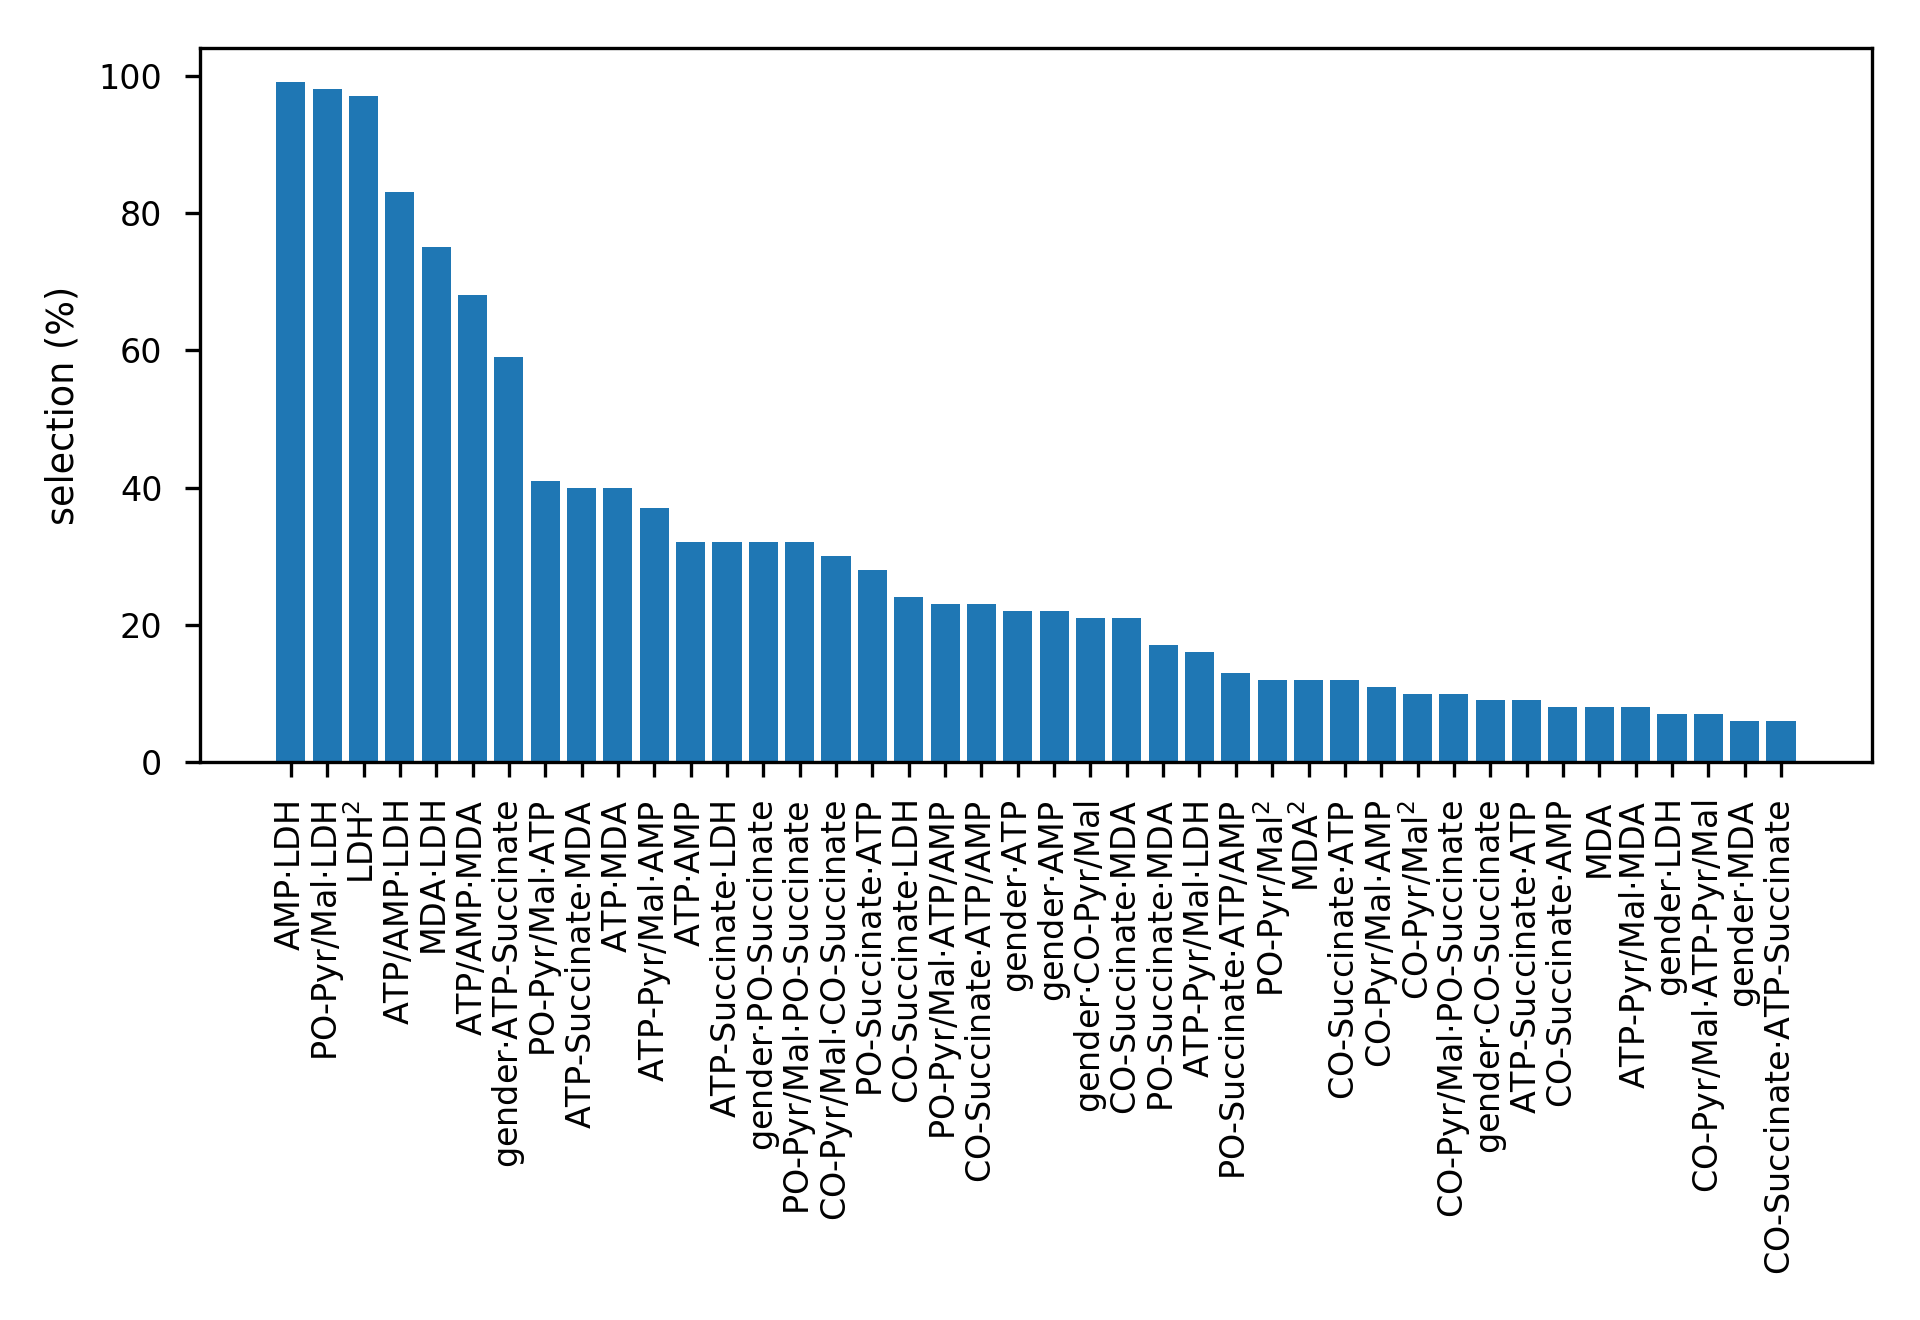
\includegraphics[width=0.8\textwidth]{part2/aging_topfeatures.png}
	\caption{The top features ... lasso ... stability selection.} \label{fig:frassoni_topfeat}
\end{figure}


\begin{figure}[]
	\centering
	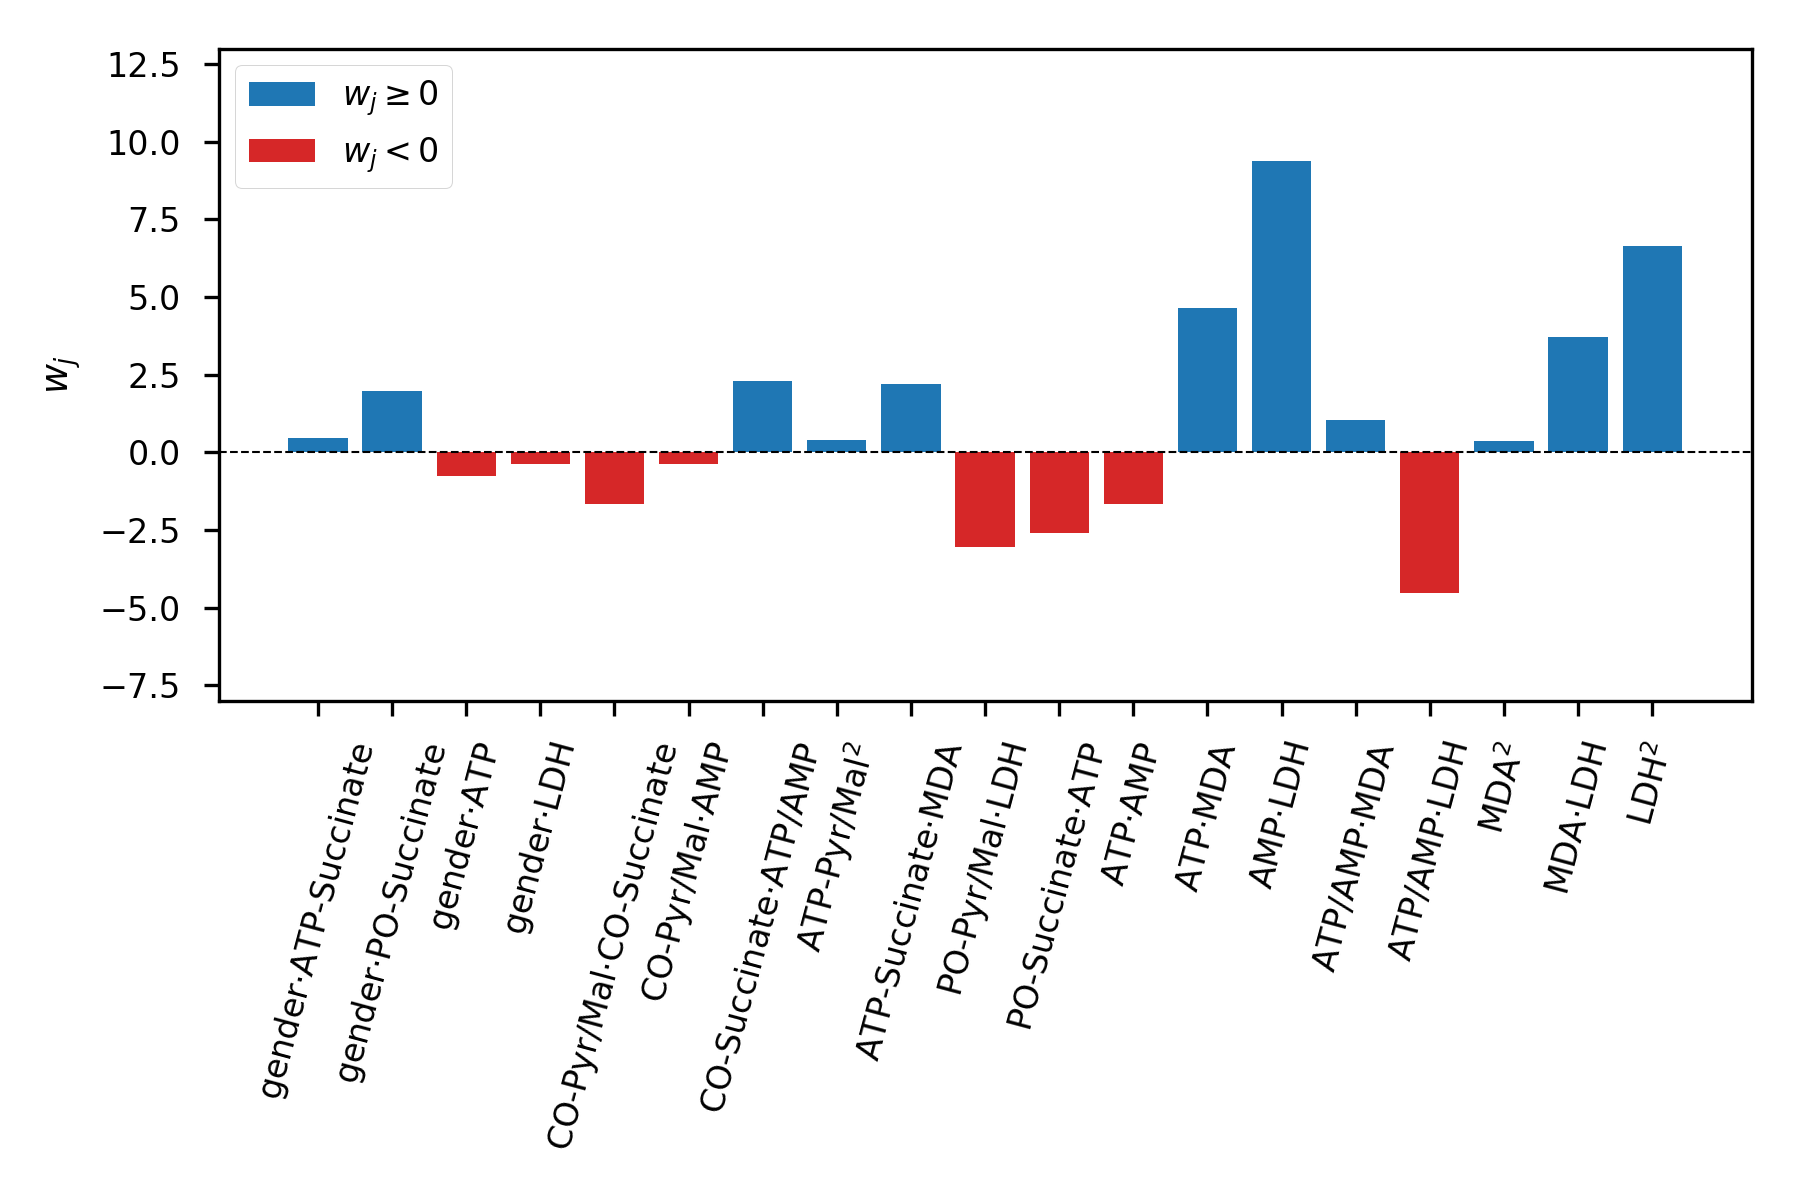
\includegraphics[width=0.8\textwidth]{part2/aging_lassopolyfeat.png}
	\caption{The top model ... lasso ....} \label{fig:frassoni_topmodel}
\end{figure}



\section{Conclusions and future works} \label{sec:frassoni_conclusions}
% CCS

future: collect more data in order to have a uniformly distributed dataset

%%